% WACV 2027 — SafeWorld / AlpaSafe trajectory-selector paper
% Based on the official WACV 2027 template (ICCV 2025 kit); upload this file
% over the template's main.tex on Overleaf (see README.md for the file map).

\documentclass[10pt,twocolumn,letterpaper]{article}

%%%%%%%%% PAPER TYPE  - PLEASE UPDATE FOR FINAL VERSION
% \usepackage[review,algorithms]{wacv}      % REVIEW version, algorithms track
\usepackage[review,applications]{wacv}      % REVIEW version, applications track
% \usepackage[review,datasets]{wacv}        % REVIEW version, datasets track
% \usepackage{wacv}                         % CAMERA-READY version
%\usepackage[pagenumbers]{wacv}             % force page numbers, e.g. arXiv

% Preamble.
% On Overleaf: the WACV template ships its own preamble.tex. Either replace it
% with this file, or keep the template's and append only the block marked
% "PAPER-SPECIFIC ADDITIONS" below (everything above that block is standard
% template fare; duplicated \usepackage of the same package without clashing
% options is harmless).

% ---- standard template packages ----
\usepackage{graphicx}
\usepackage{amsmath,amssymb}
\usepackage{xcolor}
\usepackage{subcaption}

% ============ PAPER-SPECIFIC ADDITIONS (required by sec/*.tex) ============
\usepackage{booktabs}   % \toprule/\midrule/\bottomrule in all tables
\usepackage{multirow}

% Editorial marks — must render empty/resolved before camera-ready.
\newcommand{\todo}[1]{{\color{red}[TODO: #1]}}
% Placeholder emitted by make_numbers.py for FN1 endpoints until the FN1
% analysis JSON exists; grep for \fnpending before submitting.
\newcommand{\fnpending}{{\color{red}\textbf{[FN1]}}}

% Naming macros — single point of change if we later anonymize the internal
% simulator / generator names for review.
\newcommand{\simname}{AlpaSim}          % internal closed-loop simulator
\newcommand{\vlaname}{Alpamayo-1.5}     % frozen 10B driving VLA generator
\newcommand{\headname}{SafeWorld}       % the selector head / method name

% Notation shorthands
\newcommand{\regret}{\mathrm{regret}}
\newcommand{\Ltok}{\textsc{LastToken}}
\newcommand{\Lfull}{\textsc{Full}}
\newcommand{\Lnull}{\textsc{Null}}
\newcommand{\Lgeo}{\textsc{Geometry}}


\definecolor{wacvblue}{rgb}{0.21,0.49,0.74}
\usepackage[pagebackref,breaklinks,colorlinks,allcolors=wacvblue]{hyperref}
\usepackage[capitalize]{cleveref} % must load after hyperref

%%%%%%%%% PAPER ID  - PLEASE UPDATE
\def\wacvPaperID{*****} % *** Enter the WACV Paper ID here
\def\confName{WACV}
\def\confYear{2027}

%%%%%%%%%%%%%%%%%%%%%%%%%%%%%%%%%%%%%%%%%%%%%%%%%%%%%%%%%%%%%%%%%%%%%%%%%%%%
% FN1 OUTCOME SWITCHES — flip after the FN1 study finalizes (~2026-08-10),
% then regenerate sec/numbers.tex:  python3 make_numbers.py --fn1 <analysis.json>
%   \fnonedonetrue   -> FN1 numbers are available (replaces design-only text)
%   \fnonepasstrue   -> FN1 promotion gates passed (branch A);
%                       leave false for the boundary-result branch B
%%%%%%%%%%%%%%%%%%%%%%%%%%%%%%%%%%%%%%%%%%%%%%%%%%%%%%%%%%%%%%%%%%%%%%%%%%%%
\newif\iffnonedone \fnonedonetrue
\newif\iffnonepass \fnonepassfalse

% AUTO-GENERATED by make_numbers.py -- DO NOT EDIT BY HAND.
% Sources (hash-registered records):
%   fm1_analysis: /home/qiren/alpasafe/safeworld-alpamayo/artifacts/safeworld_t26g_fm1_full_l2_matched_selector_experiment/20260803T132326Z/results/t26g_fm1_analysis.json
%   fm1_gpu_gate: /home/qiren/alpasafe/safeworld-alpamayo/artifacts/safeworld_t26g_fm1_full_l2_matched_selector_experiment/20260803T132326Z/results/t26g_fm1_gpu_gate.json
%   fn0_power: /home/qiren/alpasafe/safeworld-alpamayo/artifacts/safeworld_t26g_fn0_l3_pathway_consolidation_preregistration/20260803T210139Z/contracts/t26g_fn0_power_and_sample_size_contract.json
%   fn0_conformance: /home/qiren/alpasafe/safeworld-alpamayo/artifacts/safeworld_t26g_fn0_l3_pathway_consolidation_preregistration/20260803T210139Z/results/t26g_fn0_conformance_and_budget.json
%   e0_selector: /home/qiren/alpasafe/safeworld-alpamayo/artifacts/safeworld_t26g_e0_top_of_list_selector_resolution/20260727T042825Z/contracts/t26g_e0_selector_loss_contract.json
% Regenerate: python3 make_numbers.py [--fn1 <fn1_analysis.json>]

\newcommand{\nScenes}{173}
\newcommand{\nGroups}{519}
\newcommand{\nScoresTotal}{4{,}152}
\newcommand{\TieEps}{\ensuremath{10^{-6}}}
\newcommand{\MOneKEightRegretMean}{\ensuremath{+0.0085}}
\newcommand{\MOneKEightRegretLo}{\ensuremath{+0.0030}}
\newcommand{\MOneKEightRegretHi}{\ensuremath{+0.0143}}
\newcommand{\MOneKEightRegretCI}{\ensuremath{+0.0085\;[+0.0030,\,+0.0143]}}
\newcommand{\MOneKEightRegretBracket}{\ensuremath{[+0.0030,\,+0.0143]}}
\newcommand{\MOneKEightTopOneMean}{\ensuremath{-0.053}}
\newcommand{\MOneKEightTopOneLo}{\ensuremath{-0.082}}
\newcommand{\MOneKEightTopOneHi}{\ensuremath{-0.024}}
\newcommand{\MOneKEightTopOneCI}{\ensuremath{-0.053\;[-0.082,\,-0.024]}}
\newcommand{\MOneKEightTopOneBracket}{\ensuremath{[-0.082,\,-0.024]}}
\newcommand{\MOneKFiveRegretMean}{\ensuremath{+0.0034}}
\newcommand{\MOneKFiveRegretLo}{\ensuremath{-0.0030}}
\newcommand{\MOneKFiveRegretHi}{\ensuremath{+0.0090}}
\newcommand{\MOneKFiveRegretCI}{\ensuremath{+0.0034\;[-0.0030,\,+0.0090]}}
\newcommand{\MOneKFiveRegretBracket}{\ensuremath{[-0.0030,\,+0.0090]}}
\newcommand{\MOneKFiveTopOneMean}{\ensuremath{-0.037}}
\newcommand{\MOneKFiveTopOneLo}{\ensuremath{-0.064}}
\newcommand{\MOneKFiveTopOneHi}{\ensuremath{-0.011}}
\newcommand{\MOneKFiveTopOneCI}{\ensuremath{-0.037\;[-0.064,\,-0.011]}}
\newcommand{\MOneKFiveTopOneBracket}{\ensuremath{[-0.064,\,-0.011]}}
\newcommand{\MOneKTwoRegretMean}{\ensuremath{-0.0014}}
\newcommand{\MOneKTwoRegretLo}{\ensuremath{-0.0049}}
\newcommand{\MOneKTwoRegretHi}{\ensuremath{+0.0024}}
\newcommand{\MOneKTwoRegretCI}{\ensuremath{-0.0014\;[-0.0049,\,+0.0024]}}
\newcommand{\MOneKTwoRegretBracket}{\ensuremath{[-0.0049,\,+0.0024]}}
\newcommand{\MOneKTwoTopOneMean}{\ensuremath{-0.021}}
\newcommand{\MOneKTwoTopOneLo}{\ensuremath{-0.043}}
\newcommand{\MOneKTwoTopOneHi}{\ensuremath{-0.000}}
\newcommand{\MOneKTwoTopOneCI}{\ensuremath{-0.021\;[-0.043,\,-0.000]}}
\newcommand{\MOneKTwoTopOneBracket}{\ensuremath{[-0.043,\,-0.000]}}
\newcommand{\MOneKEightPairwiseMean}{\ensuremath{-0.033}}
\newcommand{\MOneKEightPairwiseLo}{\ensuremath{-0.048}}
\newcommand{\MOneKEightPairwiseHi}{\ensuremath{-0.018}}
\newcommand{\MOneKEightPairwiseCI}{\ensuremath{-0.033\;[-0.048,\,-0.018]}}
\newcommand{\MOneKEightPairwiseBracket}{\ensuremath{[-0.048,\,-0.018]}}
\newcommand{\MOneKEightBestVsRestMean}{\ensuremath{-0.022}}
\newcommand{\MOneKEightBestVsRestLo}{\ensuremath{-0.041}}
\newcommand{\MOneKEightBestVsRestHi}{\ensuremath{-0.004}}
\newcommand{\MOneKEightBestVsRestCI}{\ensuremath{-0.022\;[-0.041,\,-0.004]}}
\newcommand{\MOneKEightBestVsRestBracket}{\ensuremath{[-0.041,\,-0.004]}}
\newcommand{\MTwoKEightRegretMean}{\ensuremath{+0.0016}}
\newcommand{\MTwoKEightRegretLo}{\ensuremath{-0.0035}}
\newcommand{\MTwoKEightRegretHi}{\ensuremath{+0.0074}}
\newcommand{\MTwoKEightRegretCI}{\ensuremath{+0.0016\;[-0.0035,\,+0.0074]}}
\newcommand{\MTwoKEightRegretBracket}{\ensuremath{[-0.0035,\,+0.0074]}}
\newcommand{\MTwoKEightTopOneMean}{\ensuremath{+0.047}}
\newcommand{\MTwoKEightTopOneLo}{\ensuremath{+0.022}}
\newcommand{\MTwoKEightTopOneHi}{\ensuremath{+0.073}}
\newcommand{\MTwoKEightTopOneCI}{\ensuremath{+0.047\;[+0.022,\,+0.073]}}
\newcommand{\MTwoKEightTopOneBracket}{\ensuremath{[+0.022,\,+0.073]}}
\newcommand{\MTwoKFiveRegretMean}{\ensuremath{+0.0003}}
\newcommand{\MTwoKFiveRegretLo}{\ensuremath{-0.0048}}
\newcommand{\MTwoKFiveRegretHi}{\ensuremath{+0.0058}}
\newcommand{\MTwoKFiveRegretCI}{\ensuremath{+0.0003\;[-0.0048,\,+0.0058]}}
\newcommand{\MTwoKFiveRegretBracket}{\ensuremath{[-0.0048,\,+0.0058]}}
\newcommand{\MTwoKFiveTopOneMean}{\ensuremath{+0.046}}
\newcommand{\MTwoKFiveTopOneLo}{\ensuremath{+0.021}}
\newcommand{\MTwoKFiveTopOneHi}{\ensuremath{+0.071}}
\newcommand{\MTwoKFiveTopOneCI}{\ensuremath{+0.046\;[+0.021,\,+0.071]}}
\newcommand{\MTwoKFiveTopOneBracket}{\ensuremath{[+0.021,\,+0.071]}}
\newcommand{\MTwoKTwoRegretMean}{\ensuremath{-0.0002}}
\newcommand{\MTwoKTwoRegretLo}{\ensuremath{-0.0025}}
\newcommand{\MTwoKTwoRegretHi}{\ensuremath{+0.0022}}
\newcommand{\MTwoKTwoRegretCI}{\ensuremath{-0.0002\;[-0.0025,\,+0.0022]}}
\newcommand{\MTwoKTwoRegretBracket}{\ensuremath{[-0.0025,\,+0.0022]}}
\newcommand{\MTwoKTwoTopOneMean}{\ensuremath{+0.025}}
\newcommand{\MTwoKTwoTopOneLo}{\ensuremath{+0.004}}
\newcommand{\MTwoKTwoTopOneHi}{\ensuremath{+0.047}}
\newcommand{\MTwoKTwoTopOneCI}{\ensuremath{+0.025\;[+0.004,\,+0.047]}}
\newcommand{\MTwoKTwoTopOneBracket}{\ensuremath{[+0.004,\,+0.047]}}
\newcommand{\MTwoKEightPairwiseMean}{\ensuremath{+0.035}}
\newcommand{\MTwoKEightPairwiseLo}{\ensuremath{+0.022}}
\newcommand{\MTwoKEightPairwiseHi}{\ensuremath{+0.049}}
\newcommand{\MTwoKEightPairwiseCI}{\ensuremath{+0.035\;[+0.022,\,+0.049]}}
\newcommand{\MTwoKEightPairwiseBracket}{\ensuremath{[+0.022,\,+0.049]}}
\newcommand{\MTwoKEightBestVsRestMean}{\ensuremath{+0.041}}
\newcommand{\MTwoKEightBestVsRestLo}{\ensuremath{+0.022}}
\newcommand{\MTwoKEightBestVsRestHi}{\ensuremath{+0.061}}
\newcommand{\MTwoKEightBestVsRestCI}{\ensuremath{+0.041\;[+0.022,\,+0.061]}}
\newcommand{\MTwoKEightBestVsRestBracket}{\ensuremath{[+0.022,\,+0.061]}}
\newcommand{\MThreeKEightRegretMean}{\ensuremath{-0.0069}}
\newcommand{\MThreeKEightRegretLo}{\ensuremath{-0.0124}}
\newcommand{\MThreeKEightRegretHi}{\ensuremath{-0.0012}}
\newcommand{\MThreeKEightRegretCI}{\ensuremath{-0.0069\;[-0.0124,\,-0.0012]}}
\newcommand{\MThreeKEightRegretBracket}{\ensuremath{[-0.0124,\,-0.0012]}}
\newcommand{\MThreeKEightTopOneMean}{\ensuremath{+0.100}}
\newcommand{\MThreeKEightTopOneLo}{\ensuremath{+0.067}}
\newcommand{\MThreeKEightTopOneHi}{\ensuremath{+0.133}}
\newcommand{\MThreeKEightTopOneCI}{\ensuremath{+0.100\;[+0.067,\,+0.133]}}
\newcommand{\MThreeKEightTopOneBracket}{\ensuremath{[+0.067,\,+0.133]}}
\newcommand{\MThreeKFiveRegretMean}{\ensuremath{-0.0030}}
\newcommand{\MThreeKFiveRegretLo}{\ensuremath{-0.0079}}
\newcommand{\MThreeKFiveRegretHi}{\ensuremath{+0.0022}}
\newcommand{\MThreeKFiveRegretCI}{\ensuremath{-0.0030\;[-0.0079,\,+0.0022]}}
\newcommand{\MThreeKFiveRegretBracket}{\ensuremath{[-0.0079,\,+0.0022]}}
\newcommand{\MThreeKFiveTopOneMean}{\ensuremath{+0.083}}
\newcommand{\MThreeKFiveTopOneLo}{\ensuremath{+0.054}}
\newcommand{\MThreeKFiveTopOneHi}{\ensuremath{+0.113}}
\newcommand{\MThreeKFiveTopOneCI}{\ensuremath{+0.083\;[+0.054,\,+0.113]}}
\newcommand{\MThreeKFiveTopOneBracket}{\ensuremath{[+0.054,\,+0.113]}}
\newcommand{\MThreeKTwoRegretMean}{\ensuremath{+0.0012}}
\newcommand{\MThreeKTwoRegretLo}{\ensuremath{-0.0029}}
\newcommand{\MThreeKTwoRegretHi}{\ensuremath{+0.0053}}
\newcommand{\MThreeKTwoRegretCI}{\ensuremath{+0.0012\;[-0.0029,\,+0.0053]}}
\newcommand{\MThreeKTwoRegretBracket}{\ensuremath{[-0.0029,\,+0.0053]}}
\newcommand{\MThreeKTwoTopOneMean}{\ensuremath{+0.046}}
\newcommand{\MThreeKTwoTopOneLo}{\ensuremath{+0.021}}
\newcommand{\MThreeKTwoTopOneHi}{\ensuremath{+0.072}}
\newcommand{\MThreeKTwoTopOneCI}{\ensuremath{+0.046\;[+0.021,\,+0.072]}}
\newcommand{\MThreeKTwoTopOneBracket}{\ensuremath{[+0.021,\,+0.072]}}
\newcommand{\MThreeKEightPairwiseMean}{\ensuremath{+0.068}}
\newcommand{\MThreeKEightPairwiseLo}{\ensuremath{+0.051}}
\newcommand{\MThreeKEightPairwiseHi}{\ensuremath{+0.086}}
\newcommand{\MThreeKEightPairwiseCI}{\ensuremath{+0.068\;[+0.051,\,+0.086]}}
\newcommand{\MThreeKEightPairwiseBracket}{\ensuremath{[+0.051,\,+0.086]}}
\newcommand{\MThreeKEightBestVsRestMean}{\ensuremath{+0.063}}
\newcommand{\MThreeKEightBestVsRestLo}{\ensuremath{+0.042}}
\newcommand{\MThreeKEightBestVsRestHi}{\ensuremath{+0.085}}
\newcommand{\MThreeKEightBestVsRestCI}{\ensuremath{+0.063\;[+0.042,\,+0.085]}}
\newcommand{\MThreeKEightBestVsRestBracket}{\ensuremath{[+0.042,\,+0.085]}}
\newcommand{\MFourKEightRegretMean}{\ensuremath{+0.0034}}
\newcommand{\MFourKEightRegretLo}{\ensuremath{-0.0023}}
\newcommand{\MFourKEightRegretHi}{\ensuremath{+0.0092}}
\newcommand{\MFourKEightRegretCI}{\ensuremath{+0.0034\;[-0.0023,\,+0.0092]}}
\newcommand{\MFourKEightRegretBracket}{\ensuremath{[-0.0023,\,+0.0092]}}
\newcommand{\MFourKEightTopOneMean}{\ensuremath{-0.086}}
\newcommand{\MFourKEightTopOneLo}{\ensuremath{-0.122}}
\newcommand{\MFourKEightTopOneHi}{\ensuremath{-0.050}}
\newcommand{\MFourKEightTopOneCI}{\ensuremath{-0.086\;[-0.122,\,-0.050]}}
\newcommand{\MFourKEightTopOneBracket}{\ensuremath{[-0.122,\,-0.050]}}
\newcommand{\MFourKFiveRegretMean}{\ensuremath{+0.0015}}
\newcommand{\MFourKFiveRegretLo}{\ensuremath{-0.0038}}
\newcommand{\MFourKFiveRegretHi}{\ensuremath{+0.0070}}
\newcommand{\MFourKFiveRegretCI}{\ensuremath{+0.0015\;[-0.0038,\,+0.0070]}}
\newcommand{\MFourKFiveRegretBracket}{\ensuremath{[-0.0038,\,+0.0070]}}
\newcommand{\MFourKFiveTopOneMean}{\ensuremath{-0.080}}
\newcommand{\MFourKFiveTopOneLo}{\ensuremath{-0.115}}
\newcommand{\MFourKFiveTopOneHi}{\ensuremath{-0.046}}
\newcommand{\MFourKFiveTopOneCI}{\ensuremath{-0.080\;[-0.115,\,-0.046]}}
\newcommand{\MFourKFiveTopOneBracket}{\ensuremath{[-0.115,\,-0.046]}}
\newcommand{\MFourKTwoRegretMean}{\ensuremath{+0.0003}}
\newcommand{\MFourKTwoRegretLo}{\ensuremath{-0.0042}}
\newcommand{\MFourKTwoRegretHi}{\ensuremath{+0.0054}}
\newcommand{\MFourKTwoRegretCI}{\ensuremath{+0.0003\;[-0.0042,\,+0.0054]}}
\newcommand{\MFourKTwoRegretBracket}{\ensuremath{[-0.0042,\,+0.0054]}}
\newcommand{\MFourKTwoTopOneMean}{\ensuremath{-0.058}}
\newcommand{\MFourKTwoTopOneLo}{\ensuremath{-0.083}}
\newcommand{\MFourKTwoTopOneHi}{\ensuremath{-0.032}}
\newcommand{\MFourKTwoTopOneCI}{\ensuremath{-0.058\;[-0.083,\,-0.032]}}
\newcommand{\MFourKTwoTopOneBracket}{\ensuremath{[-0.083,\,-0.032]}}
\newcommand{\MFourKEightPairwiseMean}{\ensuremath{-0.051}}
\newcommand{\MFourKEightPairwiseLo}{\ensuremath{-0.073}}
\newcommand{\MFourKEightPairwiseHi}{\ensuremath{-0.029}}
\newcommand{\MFourKEightPairwiseCI}{\ensuremath{-0.051\;[-0.073,\,-0.029]}}
\newcommand{\MFourKEightPairwiseBracket}{\ensuremath{[-0.073,\,-0.029]}}
\newcommand{\MFourKEightBestVsRestMean}{\ensuremath{-0.051}}
\newcommand{\MFourKEightBestVsRestLo}{\ensuremath{-0.077}}
\newcommand{\MFourKEightBestVsRestHi}{\ensuremath{-0.026}}
\newcommand{\MFourKEightBestVsRestCI}{\ensuremath{-0.051\;[-0.077,\,-0.026]}}
\newcommand{\MFourKEightBestVsRestBracket}{\ensuremath{[-0.077,\,-0.026]}}
\newcommand{\MFiveKEightRegretMean}{\ensuremath{-0.0051}}
\newcommand{\MFiveKEightRegretLo}{\ensuremath{-0.0114}}
\newcommand{\MFiveKEightRegretHi}{\ensuremath{+0.0005}}
\newcommand{\MFiveKEightRegretCI}{\ensuremath{-0.0051\;[-0.0114,\,+0.0005]}}
\newcommand{\MFiveKEightRegretBracket}{\ensuremath{[-0.0114,\,+0.0005]}}
\newcommand{\MFiveKEightTopOneMean}{\ensuremath{-0.033}}
\newcommand{\MFiveKEightTopOneLo}{\ensuremath{-0.071}}
\newcommand{\MFiveKEightTopOneHi}{\ensuremath{+0.004}}
\newcommand{\MFiveKEightTopOneCI}{\ensuremath{-0.033\;[-0.071,\,+0.004]}}
\newcommand{\MFiveKEightTopOneBracket}{\ensuremath{[-0.071,\,+0.004]}}
\newcommand{\MFiveKFiveRegretMean}{\ensuremath{-0.0018}}
\newcommand{\MFiveKFiveRegretLo}{\ensuremath{-0.0079}}
\newcommand{\MFiveKFiveRegretHi}{\ensuremath{+0.0042}}
\newcommand{\MFiveKFiveRegretCI}{\ensuremath{-0.0018\;[-0.0079,\,+0.0042]}}
\newcommand{\MFiveKFiveRegretBracket}{\ensuremath{[-0.0079,\,+0.0042]}}
\newcommand{\MFiveKFiveTopOneMean}{\ensuremath{-0.042}}
\newcommand{\MFiveKFiveTopOneLo}{\ensuremath{-0.080}}
\newcommand{\MFiveKFiveTopOneHi}{\ensuremath{-0.006}}
\newcommand{\MFiveKFiveTopOneCI}{\ensuremath{-0.042\;[-0.080,\,-0.006]}}
\newcommand{\MFiveKFiveTopOneBracket}{\ensuremath{[-0.080,\,-0.006]}}
\newcommand{\MFiveKTwoRegretMean}{\ensuremath{+0.0016}}
\newcommand{\MFiveKTwoRegretLo}{\ensuremath{-0.0018}}
\newcommand{\MFiveKTwoRegretHi}{\ensuremath{+0.0053}}
\newcommand{\MFiveKTwoRegretCI}{\ensuremath{+0.0016\;[-0.0018,\,+0.0053]}}
\newcommand{\MFiveKTwoRegretBracket}{\ensuremath{[-0.0018,\,+0.0053]}}
\newcommand{\MFiveKTwoTopOneMean}{\ensuremath{-0.037}}
\newcommand{\MFiveKTwoTopOneLo}{\ensuremath{-0.063}}
\newcommand{\MFiveKTwoTopOneHi}{\ensuremath{-0.012}}
\newcommand{\MFiveKTwoTopOneCI}{\ensuremath{-0.037\;[-0.063,\,-0.012]}}
\newcommand{\MFiveKTwoTopOneBracket}{\ensuremath{[-0.063,\,-0.012]}}
\newcommand{\MFiveKEightPairwiseMean}{\ensuremath{-0.018}}
\newcommand{\MFiveKEightPairwiseLo}{\ensuremath{-0.040}}
\newcommand{\MFiveKEightPairwiseHi}{\ensuremath{+0.004}}
\newcommand{\MFiveKEightPairwiseCI}{\ensuremath{-0.018\;[-0.040,\,+0.004]}}
\newcommand{\MFiveKEightPairwiseBracket}{\ensuremath{[-0.040,\,+0.004]}}
\newcommand{\MFiveKEightBestVsRestMean}{\ensuremath{-0.029}}
\newcommand{\MFiveKEightBestVsRestLo}{\ensuremath{-0.056}}
\newcommand{\MFiveKEightBestVsRestHi}{\ensuremath{-0.003}}
\newcommand{\MFiveKEightBestVsRestCI}{\ensuremath{-0.029\;[-0.056,\,-0.003]}}
\newcommand{\MFiveKEightBestVsRestBracket}{\ensuremath{[-0.056,\,-0.003]}}
\newcommand{\AblWrongSceneRegretMean}{\ensuremath{+0.0007}}
\newcommand{\AblWrongSceneRegretLo}{\ensuremath{-0.0024}}
\newcommand{\AblWrongSceneRegretHi}{\ensuremath{+0.0038}}
\newcommand{\AblWrongSceneRegretCI}{\ensuremath{+0.0007\;[-0.0024,\,+0.0038]}}
\newcommand{\AblWrongSceneRegretBracket}{\ensuremath{[-0.0024,\,+0.0038]}}
\newcommand{\AblWrongSceneTopOneMean}{\ensuremath{-0.019}}
\newcommand{\AblWrongSceneTopOneLo}{\ensuremath{-0.038}}
\newcommand{\AblWrongSceneTopOneHi}{\ensuremath{-0.002}}
\newcommand{\AblWrongSceneTopOneCI}{\ensuremath{-0.019\;[-0.038,\,-0.002]}}
\newcommand{\AblWrongSceneTopOneBracket}{\ensuremath{[-0.038,\,-0.002]}}
\newcommand{\AblZeroSceneRegretMean}{\ensuremath{+0.0012}}
\newcommand{\AblZeroSceneRegretLo}{\ensuremath{-0.0020}}
\newcommand{\AblZeroSceneRegretHi}{\ensuremath{+0.0050}}
\newcommand{\AblZeroSceneRegretCI}{\ensuremath{+0.0012\;[-0.0020,\,+0.0050]}}
\newcommand{\AblZeroSceneRegretBracket}{\ensuremath{[-0.0020,\,+0.0050]}}
\newcommand{\AblZeroSceneTopOneMean}{\ensuremath{-0.024}}
\newcommand{\AblZeroSceneTopOneLo}{\ensuremath{-0.045}}
\newcommand{\AblZeroSceneTopOneHi}{\ensuremath{-0.004}}
\newcommand{\AblZeroSceneTopOneCI}{\ensuremath{-0.024\;[-0.045,\,-0.004]}}
\newcommand{\AblZeroSceneTopOneBracket}{\ensuremath{[-0.045,\,-0.004]}}
\newcommand{\AblLastTokenDiagRegretMean}{\ensuremath{-0.0008}}
\newcommand{\AblLastTokenDiagRegretLo}{\ensuremath{-0.0059}}
\newcommand{\AblLastTokenDiagRegretHi}{\ensuremath{+0.0035}}
\newcommand{\AblLastTokenDiagRegretCI}{\ensuremath{-0.0008\;[-0.0059,\,+0.0035]}}
\newcommand{\AblLastTokenDiagRegretBracket}{\ensuremath{[-0.0059,\,+0.0035]}}
\newcommand{\AblLastTokenDiagTopOneMean}{\ensuremath{-0.041}}
\newcommand{\AblLastTokenDiagTopOneLo}{\ensuremath{-0.062}}
\newcommand{\AblLastTokenDiagTopOneHi}{\ensuremath{-0.022}}
\newcommand{\AblLastTokenDiagTopOneCI}{\ensuremath{-0.041\;[-0.062,\,-0.022]}}
\newcommand{\AblLastTokenDiagTopOneBracket}{\ensuremath{[-0.062,\,-0.022]}}
\newcommand{\AbsLasttokenKEightRegret}{\ensuremath{0.0371}}
\newcommand{\AbsLasttokenKEightTopOne}{\ensuremath{0.667}}
\newcommand{\AbsLasttokenKEightPairwise}{\ensuremath{0.809}}
\newcommand{\AbsLasttokenCollisionAuroc}{\ensuremath{0.703}}
\newcommand{\AbsLasttokenAde}{\ensuremath{0.351}}
\newcommand{\AbsNullKEightRegret}{\ensuremath{0.0439}}
\newcommand{\AbsNullKEightTopOne}{\ensuremath{0.567}}
\newcommand{\AbsNullKEightPairwise}{\ensuremath{0.741}}
\newcommand{\AbsNullCollisionAuroc}{\ensuremath{0.476}}
\newcommand{\AbsNullAde}{\ensuremath{0.414}}
\newcommand{\AbsFullKEightRegret}{\ensuremath{0.0456}}
\newcommand{\AbsFullKEightTopOne}{\ensuremath{0.614}}
\newcommand{\AbsFullKEightPairwise}{\ensuremath{0.776}}
\newcommand{\AbsFullCollisionAuroc}{\ensuremath{0.566}}
\newcommand{\AbsFullAde}{\ensuremath{0.371}}
\newcommand{\AbsLegacyKEightRegret}{\ensuremath{0.0422}}
\newcommand{\AbsLegacyKEightTopOne}{\ensuremath{0.700}}
\newcommand{\AbsLegacyKEightPairwise}{\ensuremath{0.827}}
\newcommand{\AbsLegacyCollisionAuroc}{\ensuremath{0.342}}
\newcommand{\AbsLegacyAde}{\ensuremath{0.862}}
\newcommand{\AbsFullDiagKEightTopOne}{\ensuremath{0.573}}
\newcommand{\AbsFullWrongKEightTopOne}{\ensuremath{0.595}}
\newcommand{\AbsFullZeroKEightTopOne}{\ensuremath{0.590}}
\newcommand{\AuxAdeMean}{\ensuremath{+0.021}}
\newcommand{\AuxAdeLo}{\ensuremath{+0.011}}
\newcommand{\AuxAdeHi}{\ensuremath{+0.030}}
\newcommand{\AuxAdeCI}{\ensuremath{+0.021\;[+0.011,\,+0.030]}}
\newcommand{\AuxAdeBracket}{\ensuremath{[+0.011,\,+0.030]}}
\newcommand{\AuxFdeMean}{\ensuremath{-0.072}}
\newcommand{\AuxFdeLo}{\ensuremath{-0.102}}
\newcommand{\AuxFdeHi}{\ensuremath{-0.042}}
\newcommand{\AuxFdeCI}{\ensuremath{-0.072\;[-0.102,\,-0.042]}}
\newcommand{\AuxFdeBracket}{\ensuremath{[-0.102,\,-0.042]}}
\newcommand{\AuxCollisionMean}{\ensuremath{-0.137}}
\newcommand{\AuxCollisionLo}{\ensuremath{-0.245}}
\newcommand{\AuxCollisionHi}{\ensuremath{-0.031}}
\newcommand{\AuxCollisionCI}{\ensuremath{-0.137\;[-0.245,\,-0.031]}}
\newcommand{\AuxCollisionBracket}{\ensuremath{[-0.245,\,-0.031]}}
\newcommand{\AuxProgressMean}{\ensuremath{-0.035}}
\newcommand{\AuxProgressLo}{\ensuremath{-0.049}}
\newcommand{\AuxProgressHi}{\ensuremath{-0.020}}
\newcommand{\AuxProgressCI}{\ensuremath{-0.035\;[-0.049,\,-0.020]}}
\newcommand{\AuxProgressBracket}{\ensuremath{[-0.049,\,-0.020]}}
\newcommand{\AuxCollisionNScenes}{29}
\newcommand{\FnNTotal}{466}
\newcommand{\FnNExisting}{173}
\newcommand{\FnNNewPreAttrition}{293}
\newcommand{\FnNNew}{352}
\newcommand{\FnAcquisitionTotal}{525}
\newcommand{\FnMde}{\ensuremath{0.00514}}
\newcommand{\FnSdPaired}{\ensuremath{0.0396}}
\newcommand{\FnPowerAchieved}{\ensuremath{0.800}}
\newcommand{\FnPowerAtPool}{\ensuremath{0.946}}
\newcommand{\FnTopOneMde}{\ensuremath{0.033}}
\newcommand{\FnPoolRemaining}{581}
\newcommand{\EffParams}{1{,}708{,}871}
\newcommand{\EffLtMedianMs}{\ensuremath{1.19}}
\newcommand{\EffLtTailMs}{\ensuremath{1.21}}
\newcommand{\EffLtMemMb}{\ensuremath{3.5}}
\newcommand{\EffFullMedianMs}{\ensuremath{1.29}}
\newcommand{\EffFullTailMs}{\ensuremath{1.30}}
\newcommand{\EffFullMemMb}{\ensuremath{165.2}}
\newcommand{\EffTrainPeakMb}{\ensuremath{398.7}}
\newcommand{\EffMemRatio}{\ensuremath{47}}
\newcommand{\EffCeilMedianMs}{\ensuremath{10}}
\newcommand{\EffCeilTailMs}{\ensuremath{15}}
\newcommand{\EffCeilMemGb}{\ensuremath{1}}
\newcommand{\EffCeilParams}{2{,}000{,}000}
\newcommand{\SelTau}{\ensuremath{0.043}}
\newcommand{\SelCoef}{\ensuremath{0.026}}
\newcommand{\SelGradSat}{\ensuremath{24.9}}
\newcommand{\SelGradVanish}{\ensuremath{1.3\times 10^{-60}}}

% ---- FN1 (T26G-FN1) endpoints: PENDING until the FN1 analysis JSON exists ----
\newcommand{\NOneKEightRegretMean}{\ensuremath{-0.0014}}
\newcommand{\NOneKEightRegretLo}{\ensuremath{-0.0057}}
\newcommand{\NOneKEightRegretHi}{\ensuremath{+0.0028}}
\newcommand{\NOneKEightRegretCI}{\ensuremath{-0.0014\;[-0.0057,\,+0.0028]}}
\newcommand{\NOneKEightRegretBracket}{\ensuremath{[-0.0057,\,+0.0028]}}
\newcommand{\NOneKEightTopOneMean}{\ensuremath{+0.003}}
\newcommand{\NOneKEightTopOneLo}{\ensuremath{-0.020}}
\newcommand{\NOneKEightTopOneHi}{\ensuremath{+0.028}}
\newcommand{\NOneKEightTopOneCI}{\ensuremath{+0.003\;[-0.020,\,+0.028]}}
\newcommand{\NOneKEightTopOneBracket}{\ensuremath{[-0.020,\,+0.028]}}
\newcommand{\NOneKFiveRegretMean}{\ensuremath{+0.0013}}
\newcommand{\NOneKFiveRegretLo}{\ensuremath{-0.0023}}
\newcommand{\NOneKFiveRegretHi}{\ensuremath{+0.0048}}
\newcommand{\NOneKFiveRegretCI}{\ensuremath{+0.0013\;[-0.0023,\,+0.0048]}}
\newcommand{\NOneKFiveRegretBracket}{\ensuremath{[-0.0023,\,+0.0048]}}
\newcommand{\NOneKFiveTopOneMean}{\ensuremath{+0.009}}
\newcommand{\NOneKFiveTopOneLo}{\ensuremath{-0.012}}
\newcommand{\NOneKFiveTopOneHi}{\ensuremath{+0.031}}
\newcommand{\NOneKFiveTopOneCI}{\ensuremath{+0.009\;[-0.012,\,+0.031]}}
\newcommand{\NOneKFiveTopOneBracket}{\ensuremath{[-0.012,\,+0.031]}}
\newcommand{\NOneKTwoRegretMean}{\ensuremath{+0.0012}}
\newcommand{\NOneKTwoRegretLo}{\ensuremath{-0.0016}}
\newcommand{\NOneKTwoRegretHi}{\ensuremath{+0.0040}}
\newcommand{\NOneKTwoRegretCI}{\ensuremath{+0.0012\;[-0.0016,\,+0.0040]}}
\newcommand{\NOneKTwoRegretBracket}{\ensuremath{[-0.0016,\,+0.0040]}}
\newcommand{\NOneKTwoTopOneMean}{\ensuremath{+0.021}}
\newcommand{\NOneKTwoTopOneLo}{\ensuremath{+0.006}}
\newcommand{\NOneKTwoTopOneHi}{\ensuremath{+0.036}}
\newcommand{\NOneKTwoTopOneCI}{\ensuremath{+0.021\;[+0.006,\,+0.036]}}
\newcommand{\NOneKTwoTopOneBracket}{\ensuremath{[+0.006,\,+0.036]}}
\newcommand{\NOneKEightPairwiseMean}{\ensuremath{+0.050}}
\newcommand{\NOneKEightPairwiseLo}{\ensuremath{+0.031}}
\newcommand{\NOneKEightPairwiseHi}{\ensuremath{+0.071}}
\newcommand{\NOneKEightPairwiseCI}{\ensuremath{+0.050\;[+0.031,\,+0.071]}}
\newcommand{\NOneKEightPairwiseBracket}{\ensuremath{[+0.031,\,+0.071]}}
\newcommand{\NOneKEightBestVsRestMean}{\ensuremath{+0.052}}
\newcommand{\NOneKEightBestVsRestLo}{\ensuremath{+0.031}}
\newcommand{\NOneKEightBestVsRestHi}{\ensuremath{+0.074}}
\newcommand{\NOneKEightBestVsRestCI}{\ensuremath{+0.052\;[+0.031,\,+0.074]}}
\newcommand{\NOneKEightBestVsRestBracket}{\ensuremath{[+0.031,\,+0.074]}}
\newcommand{\NTwoKEightRegretMean}{\ensuremath{-0.0129}}
\newcommand{\NTwoKEightRegretLo}{\ensuremath{-0.0173}}
\newcommand{\NTwoKEightRegretHi}{\ensuremath{-0.0086}}
\newcommand{\NTwoKEightRegretCI}{\ensuremath{-0.0129\;[-0.0173,\,-0.0086]}}
\newcommand{\NTwoKEightRegretBracket}{\ensuremath{[-0.0173,\,-0.0086]}}
\newcommand{\NTwoKEightTopOneMean}{\ensuremath{+0.112}}
\newcommand{\NTwoKEightTopOneLo}{\ensuremath{+0.094}}
\newcommand{\NTwoKEightTopOneHi}{\ensuremath{+0.130}}
\newcommand{\NTwoKEightTopOneCI}{\ensuremath{+0.112\;[+0.094,\,+0.130]}}
\newcommand{\NTwoKEightTopOneBracket}{\ensuremath{[+0.094,\,+0.130]}}
\newcommand{\NTwoKFiveRegretMean}{\ensuremath{-0.0088}}
\newcommand{\NTwoKFiveRegretLo}{\ensuremath{-0.0126}}
\newcommand{\NTwoKFiveRegretHi}{\ensuremath{-0.0052}}
\newcommand{\NTwoKFiveRegretCI}{\ensuremath{-0.0088\;[-0.0126,\,-0.0052]}}
\newcommand{\NTwoKFiveRegretBracket}{\ensuremath{[-0.0126,\,-0.0052]}}
\newcommand{\NTwoKFiveTopOneMean}{\ensuremath{+0.110}}
\newcommand{\NTwoKFiveTopOneLo}{\ensuremath{+0.093}}
\newcommand{\NTwoKFiveTopOneHi}{\ensuremath{+0.127}}
\newcommand{\NTwoKFiveTopOneCI}{\ensuremath{+0.110\;[+0.093,\,+0.127]}}
\newcommand{\NTwoKFiveTopOneBracket}{\ensuremath{[+0.093,\,+0.127]}}
\newcommand{\NTwoKTwoRegretMean}{\ensuremath{-0.0060}}
\newcommand{\NTwoKTwoRegretLo}{\ensuremath{-0.0092}}
\newcommand{\NTwoKTwoRegretHi}{\ensuremath{-0.0030}}
\newcommand{\NTwoKTwoRegretCI}{\ensuremath{-0.0060\;[-0.0092,\,-0.0030]}}
\newcommand{\NTwoKTwoRegretBracket}{\ensuremath{[-0.0092,\,-0.0030]}}
\newcommand{\NTwoKTwoTopOneMean}{\ensuremath{+0.073}}
\newcommand{\NTwoKTwoTopOneLo}{\ensuremath{+0.060}}
\newcommand{\NTwoKTwoTopOneHi}{\ensuremath{+0.087}}
\newcommand{\NTwoKTwoTopOneCI}{\ensuremath{+0.073\;[+0.060,\,+0.087]}}
\newcommand{\NTwoKTwoTopOneBracket}{\ensuremath{[+0.060,\,+0.087]}}
\newcommand{\NTwoKEightPairwiseMean}{\ensuremath{+0.068}}
\newcommand{\NTwoKEightPairwiseLo}{\ensuremath{+0.060}}
\newcommand{\NTwoKEightPairwiseHi}{\ensuremath{+0.076}}
\newcommand{\NTwoKEightPairwiseCI}{\ensuremath{+0.068\;[+0.060,\,+0.076]}}
\newcommand{\NTwoKEightPairwiseBracket}{\ensuremath{[+0.060,\,+0.076]}}
\newcommand{\NTwoKEightBestVsRestMean}{\ensuremath{+0.055}}
\newcommand{\NTwoKEightBestVsRestLo}{\ensuremath{+0.044}}
\newcommand{\NTwoKEightBestVsRestHi}{\ensuremath{+0.065}}
\newcommand{\NTwoKEightBestVsRestCI}{\ensuremath{+0.055\;[+0.044,\,+0.065]}}
\newcommand{\NTwoKEightBestVsRestBracket}{\ensuremath{[+0.044,\,+0.065]}}
\newcommand{\NThreeKEightRegretMean}{\ensuremath{+0.0029}}
\newcommand{\NThreeKEightRegretLo}{\ensuremath{+0.0005}}
\newcommand{\NThreeKEightRegretHi}{\ensuremath{+0.0056}}
\newcommand{\NThreeKEightRegretCI}{\ensuremath{+0.0029\;[+0.0005,\,+0.0056]}}
\newcommand{\NThreeKEightRegretBracket}{\ensuremath{[+0.0005,\,+0.0056]}}
\newcommand{\NThreeKEightTopOneMean}{\ensuremath{-0.000}}
\newcommand{\NThreeKEightTopOneLo}{\ensuremath{-0.012}}
\newcommand{\NThreeKEightTopOneHi}{\ensuremath{+0.011}}
\newcommand{\NThreeKEightTopOneCI}{\ensuremath{-0.000\;[-0.012,\,+0.011]}}
\newcommand{\NThreeKEightTopOneBracket}{\ensuremath{[-0.012,\,+0.011]}}
\newcommand{\NThreeKFiveRegretMean}{\ensuremath{+0.0014}}
\newcommand{\NThreeKFiveRegretLo}{\ensuremath{-0.0005}}
\newcommand{\NThreeKFiveRegretHi}{\ensuremath{+0.0035}}
\newcommand{\NThreeKFiveRegretCI}{\ensuremath{+0.0014\;[-0.0005,\,+0.0035]}}
\newcommand{\NThreeKFiveRegretBracket}{\ensuremath{[-0.0005,\,+0.0035]}}
\newcommand{\NThreeKFiveTopOneMean}{\ensuremath{+0.003}}
\newcommand{\NThreeKFiveTopOneLo}{\ensuremath{-0.008}}
\newcommand{\NThreeKFiveTopOneHi}{\ensuremath{+0.014}}
\newcommand{\NThreeKFiveTopOneCI}{\ensuremath{+0.003\;[-0.008,\,+0.014]}}
\newcommand{\NThreeKFiveTopOneBracket}{\ensuremath{[-0.008,\,+0.014]}}
\newcommand{\NThreeKTwoRegretMean}{\ensuremath{+0.0010}}
\newcommand{\NThreeKTwoRegretLo}{\ensuremath{-0.0009}}
\newcommand{\NThreeKTwoRegretHi}{\ensuremath{+0.0030}}
\newcommand{\NThreeKTwoRegretCI}{\ensuremath{+0.0010\;[-0.0009,\,+0.0030]}}
\newcommand{\NThreeKTwoRegretBracket}{\ensuremath{[-0.0009,\,+0.0030]}}
\newcommand{\NThreeKTwoTopOneMean}{\ensuremath{-0.003}}
\newcommand{\NThreeKTwoTopOneLo}{\ensuremath{-0.012}}
\newcommand{\NThreeKTwoTopOneHi}{\ensuremath{+0.005}}
\newcommand{\NThreeKTwoTopOneCI}{\ensuremath{-0.003\;[-0.012,\,+0.005]}}
\newcommand{\NThreeKTwoTopOneBracket}{\ensuremath{[-0.012,\,+0.005]}}
\newcommand{\NThreeKEightPairwiseMean}{\ensuremath{+0.004}}
\newcommand{\NThreeKEightPairwiseLo}{\ensuremath{-0.000}}
\newcommand{\NThreeKEightPairwiseHi}{\ensuremath{+0.008}}
\newcommand{\NThreeKEightPairwiseCI}{\ensuremath{+0.004\;[-0.000,\,+0.008]}}
\newcommand{\NThreeKEightPairwiseBracket}{\ensuremath{[-0.000,\,+0.008]}}
\newcommand{\NThreeKEightBestVsRestMean}{\ensuremath{+0.005}}
\newcommand{\NThreeKEightBestVsRestLo}{\ensuremath{-0.001}}
\newcommand{\NThreeKEightBestVsRestHi}{\ensuremath{+0.010}}
\newcommand{\NThreeKEightBestVsRestCI}{\ensuremath{+0.005\;[-0.001,\,+0.010]}}
\newcommand{\NThreeKEightBestVsRestBracket}{\ensuremath{[-0.001,\,+0.010]}}
\newcommand{\NFourKEightRegretMean}{\ensuremath{-0.0014}}
\newcommand{\NFourKEightRegretLo}{\ensuremath{-0.0057}}
\newcommand{\NFourKEightRegretHi}{\ensuremath{+0.0028}}
\newcommand{\NFourKEightRegretCI}{\ensuremath{-0.0014\;[-0.0057,\,+0.0028]}}
\newcommand{\NFourKEightRegretBracket}{\ensuremath{[-0.0057,\,+0.0028]}}
\newcommand{\NFourKEightTopOneMean}{\ensuremath{+0.003}}
\newcommand{\NFourKEightTopOneLo}{\ensuremath{-0.020}}
\newcommand{\NFourKEightTopOneHi}{\ensuremath{+0.028}}
\newcommand{\NFourKEightTopOneCI}{\ensuremath{+0.003\;[-0.020,\,+0.028]}}
\newcommand{\NFourKEightTopOneBracket}{\ensuremath{[-0.020,\,+0.028]}}
\newcommand{\NFourKFiveRegretMean}{\ensuremath{+0.0013}}
\newcommand{\NFourKFiveRegretLo}{\ensuremath{-0.0023}}
\newcommand{\NFourKFiveRegretHi}{\ensuremath{+0.0048}}
\newcommand{\NFourKFiveRegretCI}{\ensuremath{+0.0013\;[-0.0023,\,+0.0048]}}
\newcommand{\NFourKFiveRegretBracket}{\ensuremath{[-0.0023,\,+0.0048]}}
\newcommand{\NFourKFiveTopOneMean}{\ensuremath{+0.009}}
\newcommand{\NFourKFiveTopOneLo}{\ensuremath{-0.012}}
\newcommand{\NFourKFiveTopOneHi}{\ensuremath{+0.031}}
\newcommand{\NFourKFiveTopOneCI}{\ensuremath{+0.009\;[-0.012,\,+0.031]}}
\newcommand{\NFourKFiveTopOneBracket}{\ensuremath{[-0.012,\,+0.031]}}
\newcommand{\NFourKTwoRegretMean}{\ensuremath{+0.0012}}
\newcommand{\NFourKTwoRegretLo}{\ensuremath{-0.0016}}
\newcommand{\NFourKTwoRegretHi}{\ensuremath{+0.0040}}
\newcommand{\NFourKTwoRegretCI}{\ensuremath{+0.0012\;[-0.0016,\,+0.0040]}}
\newcommand{\NFourKTwoRegretBracket}{\ensuremath{[-0.0016,\,+0.0040]}}
\newcommand{\NFourKTwoTopOneMean}{\ensuremath{+0.021}}
\newcommand{\NFourKTwoTopOneLo}{\ensuremath{+0.006}}
\newcommand{\NFourKTwoTopOneHi}{\ensuremath{+0.036}}
\newcommand{\NFourKTwoTopOneCI}{\ensuremath{+0.021\;[+0.006,\,+0.036]}}
\newcommand{\NFourKTwoTopOneBracket}{\ensuremath{[+0.006,\,+0.036]}}
\newcommand{\NFourKEightPairwiseMean}{\ensuremath{+0.050}}
\newcommand{\NFourKEightPairwiseLo}{\ensuremath{+0.031}}
\newcommand{\NFourKEightPairwiseHi}{\ensuremath{+0.071}}
\newcommand{\NFourKEightPairwiseCI}{\ensuremath{+0.050\;[+0.031,\,+0.071]}}
\newcommand{\NFourKEightPairwiseBracket}{\ensuremath{[+0.031,\,+0.071]}}
\newcommand{\NFourKEightBestVsRestMean}{\ensuremath{+0.052}}
\newcommand{\NFourKEightBestVsRestLo}{\ensuremath{+0.031}}
\newcommand{\NFourKEightBestVsRestHi}{\ensuremath{+0.074}}
\newcommand{\NFourKEightBestVsRestCI}{\ensuremath{+0.052\;[+0.031,\,+0.074]}}
\newcommand{\NFourKEightBestVsRestBracket}{\ensuremath{[+0.031,\,+0.074]}}
\newcommand{\NOneSelKEightRegretMean}{\ensuremath{+0.0016}}
\newcommand{\NOneSelKEightRegretLo}{\ensuremath{-0.0022}}
\newcommand{\NOneSelKEightRegretHi}{\ensuremath{+0.0054}}
\newcommand{\NOneSelKEightRegretCI}{\ensuremath{+0.0016\;[-0.0022,\,+0.0054]}}
\newcommand{\NOneSelKEightRegretBracket}{\ensuremath{[-0.0022,\,+0.0054]}}
\newcommand{\NOneSelKEightTopOneMean}{\ensuremath{+0.003}}
\newcommand{\NOneSelKEightTopOneLo}{\ensuremath{-0.020}}
\newcommand{\NOneSelKEightTopOneHi}{\ensuremath{+0.027}}
\newcommand{\NOneSelKEightTopOneCI}{\ensuremath{+0.003\;[-0.020,\,+0.027]}}
\newcommand{\NOneSelKEightTopOneBracket}{\ensuremath{[-0.020,\,+0.027]}}
\newcommand{\NOneSelKFiveRegretMean}{\ensuremath{+0.0027}}
\newcommand{\NOneSelKFiveRegretLo}{\ensuremath{-0.0008}}
\newcommand{\NOneSelKFiveRegretHi}{\ensuremath{+0.0063}}
\newcommand{\NOneSelKFiveRegretCI}{\ensuremath{+0.0027\;[-0.0008,\,+0.0063]}}
\newcommand{\NOneSelKFiveRegretBracket}{\ensuremath{[-0.0008,\,+0.0063]}}
\newcommand{\NOneSelKFiveTopOneMean}{\ensuremath{+0.012}}
\newcommand{\NOneSelKFiveTopOneLo}{\ensuremath{-0.008}}
\newcommand{\NOneSelKFiveTopOneHi}{\ensuremath{+0.033}}
\newcommand{\NOneSelKFiveTopOneCI}{\ensuremath{+0.012\;[-0.008,\,+0.033]}}
\newcommand{\NOneSelKFiveTopOneBracket}{\ensuremath{[-0.008,\,+0.033]}}
\newcommand{\NOneSelKTwoRegretMean}{\ensuremath{+0.0022}}
\newcommand{\NOneSelKTwoRegretLo}{\ensuremath{-0.0005}}
\newcommand{\NOneSelKTwoRegretHi}{\ensuremath{+0.0051}}
\newcommand{\NOneSelKTwoRegretCI}{\ensuremath{+0.0022\;[-0.0005,\,+0.0051]}}
\newcommand{\NOneSelKTwoRegretBracket}{\ensuremath{[-0.0005,\,+0.0051]}}
\newcommand{\NOneSelKTwoTopOneMean}{\ensuremath{+0.018}}
\newcommand{\NOneSelKTwoTopOneLo}{\ensuremath{+0.003}}
\newcommand{\NOneSelKTwoTopOneHi}{\ensuremath{+0.032}}
\newcommand{\NOneSelKTwoTopOneCI}{\ensuremath{+0.018\;[+0.003,\,+0.032]}}
\newcommand{\NOneSelKTwoTopOneBracket}{\ensuremath{[+0.003,\,+0.032]}}
\newcommand{\NOneSelKEightPairwiseMean}{\ensuremath{+0.055}}
\newcommand{\NOneSelKEightPairwiseLo}{\ensuremath{+0.036}}
\newcommand{\NOneSelKEightPairwiseHi}{\ensuremath{+0.075}}
\newcommand{\NOneSelKEightPairwiseCI}{\ensuremath{+0.055\;[+0.036,\,+0.075]}}
\newcommand{\NOneSelKEightPairwiseBracket}{\ensuremath{[+0.036,\,+0.075]}}
\newcommand{\NOneSelKEightBestVsRestMean}{\ensuremath{+0.057}}
\newcommand{\NOneSelKEightBestVsRestLo}{\ensuremath{+0.036}}
\newcommand{\NOneSelKEightBestVsRestHi}{\ensuremath{+0.078}}
\newcommand{\NOneSelKEightBestVsRestCI}{\ensuremath{+0.057\;[+0.036,\,+0.078]}}
\newcommand{\NOneSelKEightBestVsRestBracket}{\ensuremath{[+0.036,\,+0.078]}}
\newcommand{\NTwoSelKEightRegretMean}{\ensuremath{-0.0100}}
\newcommand{\NTwoSelKEightRegretLo}{\ensuremath{-0.0140}}
\newcommand{\NTwoSelKEightRegretHi}{\ensuremath{-0.0060}}
\newcommand{\NTwoSelKEightRegretCI}{\ensuremath{-0.0100\;[-0.0140,\,-0.0060]}}
\newcommand{\NTwoSelKEightRegretBracket}{\ensuremath{[-0.0140,\,-0.0060]}}
\newcommand{\NTwoSelKEightTopOneMean}{\ensuremath{+0.112}}
\newcommand{\NTwoSelKEightTopOneLo}{\ensuremath{+0.094}}
\newcommand{\NTwoSelKEightTopOneHi}{\ensuremath{+0.130}}
\newcommand{\NTwoSelKEightTopOneCI}{\ensuremath{+0.112\;[+0.094,\,+0.130]}}
\newcommand{\NTwoSelKEightTopOneBracket}{\ensuremath{[+0.094,\,+0.130]}}
\newcommand{\NTwoSelKFiveRegretMean}{\ensuremath{-0.0074}}
\newcommand{\NTwoSelKFiveRegretLo}{\ensuremath{-0.0108}}
\newcommand{\NTwoSelKFiveRegretHi}{\ensuremath{-0.0040}}
\newcommand{\NTwoSelKFiveRegretCI}{\ensuremath{-0.0074\;[-0.0108,\,-0.0040]}}
\newcommand{\NTwoSelKFiveRegretBracket}{\ensuremath{[-0.0108,\,-0.0040]}}
\newcommand{\NTwoSelKFiveTopOneMean}{\ensuremath{+0.113}}
\newcommand{\NTwoSelKFiveTopOneLo}{\ensuremath{+0.096}}
\newcommand{\NTwoSelKFiveTopOneHi}{\ensuremath{+0.129}}
\newcommand{\NTwoSelKFiveTopOneCI}{\ensuremath{+0.113\;[+0.096,\,+0.129]}}
\newcommand{\NTwoSelKFiveTopOneBracket}{\ensuremath{[+0.096,\,+0.129]}}
\newcommand{\NTwoSelKTwoRegretMean}{\ensuremath{-0.0050}}
\newcommand{\NTwoSelKTwoRegretLo}{\ensuremath{-0.0077}}
\newcommand{\NTwoSelKTwoRegretHi}{\ensuremath{-0.0026}}
\newcommand{\NTwoSelKTwoRegretCI}{\ensuremath{-0.0050\;[-0.0077,\,-0.0026]}}
\newcommand{\NTwoSelKTwoRegretBracket}{\ensuremath{[-0.0077,\,-0.0026]}}
\newcommand{\NTwoSelKTwoTopOneMean}{\ensuremath{+0.070}}
\newcommand{\NTwoSelKTwoTopOneLo}{\ensuremath{+0.056}}
\newcommand{\NTwoSelKTwoTopOneHi}{\ensuremath{+0.083}}
\newcommand{\NTwoSelKTwoTopOneCI}{\ensuremath{+0.070\;[+0.056,\,+0.083]}}
\newcommand{\NTwoSelKTwoTopOneBracket}{\ensuremath{[+0.056,\,+0.083]}}
\newcommand{\NTwoSelKEightPairwiseMean}{\ensuremath{+0.072}}
\newcommand{\NTwoSelKEightPairwiseLo}{\ensuremath{+0.065}}
\newcommand{\NTwoSelKEightPairwiseHi}{\ensuremath{+0.079}}
\newcommand{\NTwoSelKEightPairwiseCI}{\ensuremath{+0.072\;[+0.065,\,+0.079]}}
\newcommand{\NTwoSelKEightPairwiseBracket}{\ensuremath{[+0.065,\,+0.079]}}
\newcommand{\NTwoSelKEightBestVsRestMean}{\ensuremath{+0.060}}
\newcommand{\NTwoSelKEightBestVsRestLo}{\ensuremath{+0.050}}
\newcommand{\NTwoSelKEightBestVsRestHi}{\ensuremath{+0.070}}
\newcommand{\NTwoSelKEightBestVsRestCI}{\ensuremath{+0.060\;[+0.050,\,+0.070]}}
\newcommand{\NTwoSelKEightBestVsRestBracket}{\ensuremath{[+0.050,\,+0.070]}}
\newcommand{\FnOneNScenes}{525}
 % AUTO-GENERATED numeric macros — never hand-edit

%%%%%%%%% TITLE
% Alternatives considered (outline §0):
%  1. Your Planner Already Knows: Frozen VLA Representations as Amortized
%     Trajectory Evaluators
%  3. SafeWorld: Amortized Online Trajectory Evaluation without a World Model
\title{One Token Is Enough: Trajectory Selection\\ from a Frozen Driving VLA's Prefill State}

%%%%%%%%% AUTHORS - anonymous for review
\author{Anonymous WACV submission\\
Paper ID \wacvPaperID}

\begin{document}
\maketitle
\begin{abstract}
End-to-end planners emit $K$ candidate trajectories per decision, yet deployment executes exactly one.
The community's reporting convention, minADE@$K$, silently assumes an oracle makes that choice, so the gap between reported potential and deployed behavior---the \emph{selected regret}---goes largely unmeasured.
Prior online trajectory evaluation closes this gap with explicit imagination: a purpose-trained BEV world model rolls out every candidate's future before scoring it.
We show that, for a strong driving VLA, the required scene knowledge has \emph{already been computed} by the generator itself.
The last hidden token of the frozen \vlaname{} (10B) prompt prefill---a byproduct of producing the candidates---read by a \EffParams-parameter decomposed value head in \EffLtMedianMs~ms, carries a causally verified, prospectively replicated selection signal: on \nScenes{} untouched scenes, selected regret improves by \MThreeKEightRegretCI{} and tie-aware top-1 agreement by \MThreeKEightTopOneCI{} (95\% CIs) over a parameter-matched scene-blind control, and wrong-scene and zeroed-representation ablations degrade selection.
Surprisingly, reading the \emph{full} 3{,}086-token prefill sequence is CI-supported \emph{worse} than its own last row under matched capacity (regret \MOneKEightRegretCI; top-1 \MOneKEightTopOneCI).
\iffnonedone
  \iffnonepass
    In an adequately powered ($1-\beta=0.80$, $N=\FnNTotal$) preregistered comparison, the representation-based selector further surpasses a trained trajectory-geometry baseline on selected regret (\NOneKEightRegretCI) without ceding top-1 agreement.
  \else
    In an adequately powered ($1-\beta=0.80$, $N=\FnNTotal$) preregistered comparison against a trained trajectory-geometry baseline, the representation adds signal but does not displace the tuned incumbent (regret \NOneKEightRegretCI), a boundary result that delimits when representation reuse pays.
  \fi
\else
  A preregistered comparison against a trained trajectory-geometry incumbent, powered at $1-\beta=0.80$ for the observed effect ($N=\FnNTotal$ scenes), completes the program. % pre-FN1 placeholder sentence
\fi
All studies are preregistered with outcome-blind frozen gates, analyzed with paired scene bootstrap CIs, and guarded by a sealed, never-opened confirmation cohort.
\end{abstract}

\section{Introduction}
\label{sec:intro}

Modern end-to-end driving stacks are multi-modal by construction: given a scene, the planner proposes $K$ candidate trajectories, and the vehicle executes one of them.
The field's dominant reporting convention, minADE@$K$ and its closed-loop analogues, scores the \emph{best} of the $K$ candidates---implicitly assuming an oracle selector that deployment does not have.
What the vehicle actually achieves is set by the candidate it \emph{selects}; the difference between the oracle's outcome and the selected outcome is the \emph{selected regret}, and it is the quantity this paper measures, models, and reduces.
Under a strong 10B-parameter driving VLA generator with $K{=}8$ sampled candidates, we find the selected regret of a trained geometry-only selector is \AbsLegacyKEightRegret{} official-score points per scene (scale $[0,1]$), against an oracle gap of zero---small in absolute terms, but persistent, and invisible to minADE-style reporting.

One route to closing this gap is \emph{explicit imagination}.
WoTE~\cite{li2025wote} trains a BEV world model alongside the planner, autoregressively imagines each candidate's future BEV state, and scores the imagined futures with imitation and simulation-based submetric rewards.
This buys online evaluation at the cost of a purpose-trained world model, per-candidate rollout compute at inference time, and supervision plumbed from simulator submetrics.

This paper asks the opposite question: \emph{does the generator's own forward pass already contain the scene knowledge a selector needs?}
The intuition is that a driving VLA trained to produce good trajectories must internally represent where hazards are, which maneuvers are viable, and how the scene constrains them---an \emph{amortized} form of the same consequence knowledge a world model would compute online.
If that knowledge is readable from activations the planner computes anyway, online evaluation becomes representation \emph{reuse}: zero VLA training, zero inference-time rollouts, and a selector head small enough to be free at deployment.

Concretely, we capture the final-layer hidden states of the frozen VLA's prompt prefill \emph{during the same forward pass that generates the candidates}---the candidates and the representation are provably co-produced (the pooled scene vector is bit-exactly the last row of the captured sequence, hash-verified at capture time; \cref{sec:capture}).
A \EffParams-parameter decomposed value head (\cref{sec:head}) reads this representation and scores each candidate independently in \EffLtMedianMs~ms for all $K{=}8$, with \EffLtMemMb~MB peak incremental memory.

Three findings structure our results.
\textbf{First}, the frozen representation carries a real, scene-specific, causally verified selection signal: on \nScenes{} prospectively frozen, never-before-touched scenes, the representation-informed head beats a parameter-matched scene-blind control on selected regret (\MThreeKEightRegretCI) and tie-aware top-1 agreement (\MThreeKEightTopOneCI), while wrong-scene substitution and representation zeroing degrade selection (\cref{sec:res-signal}).
\textbf{Second}, and counterintuitively, \emph{more context hurts}: a matched-capacity reader given the full $3{,}086\times4{,}096$ prefill sequence is CI-supported \emph{worse} than the same architecture reading only the last token (regret \MOneKEightRegretCI, top-1 \MOneKEightTopOneCI; \cref{sec:res-onetoken}).
The generator has already summarized the scene into its terminal prefill state; re-reading its full working memory dilutes the signal under a fixed parameter budget.
\textbf{Third}, effects of this size demand statistical care the area rarely applies.
Every confirmatory study in this paper was preregistered with frozen decision gates before outcomes existed; endpoints use paired scene bootstrap confidence intervals; cohorts advance on a ladder from development scenes to prospectively frozen untouched scenes to a sealed confirmation set that is never opened until a winner is frozen; and every number in this paper is machine-read from hash-locked result records (\cref{sec:program}).
\iffnonedone\else
The program culminates in a comparison against the trained geometry incumbent that is \emph{adequately powered by design}: the sample size ($N=\FnNTotal$ scenes) was derived from the locked pilot effect (MDE $\FnMde$, paired SD $\FnSdPaired$) to reach $1-\beta=\FnPowerAchieved$ at two-sided $\alpha=0.05$.
\fi

Our contributions are:
\begin{itemize}
  \item \textbf{C1 --- Same-prefill capture and an open evaluation program.} A capture protocol that provably ties the reused representation to the exact forward pass that produced the candidates, embedded in an evaluation design (preregistration, frozen gates, cohort ladder, causal ablations, sealed confirmation) that we argue should become standard for selector claims (\cref{sec:capture,sec:program}).
  \item \textbf{C2 --- Positive result.} The frozen VLA's last prefill token supports scene-specific trajectory selection with CI-supported gains on both primary endpoints, replicated prospectively on untouched scenes and causally verified by ablation (\cref{sec:res-signal}).
  \item \textbf{C3 --- Negative result.} Under matched capacity, the full prefill sequence is CI-supported worse than its last token alone---a ``more context hurts'' finding with direct architectural consequences for representation-reuse selectors (\cref{sec:res-onetoken}).
  \item \textbf{C4 --- Powered incumbent verdict.}
  \iffnonedone
    \iffnonepass
      At $1-\beta=0.80$ power, the representation-based selector surpasses the tuned trajectory-geometry incumbent on the promoting endpoint with preregistered non-inferiority on the others (\cref{sec:res-incumbent}).
    \else
      At $1-\beta=0.80$ power, the representation-based selector does \emph{not} displace the tuned trajectory-geometry incumbent; we report this as a clean, adequately powered boundary on when representation reuse pays, together with the conditions under which the representation \emph{does} add value (\cref{sec:res-incumbent}).
    \fi
  \else
    An adequately powered ($N=\FnNTotal$, $1-\beta=0.80$), preregistered verdict on whether the reused representation displaces a tuned trajectory-geometry incumbent (\cref{sec:res-incumbent}). \todo{FN1 lands $\sim$Aug 10; both outcome branches are pre-written.}
  \fi
\end{itemize}

\begin{figure}[t]
  \centering
  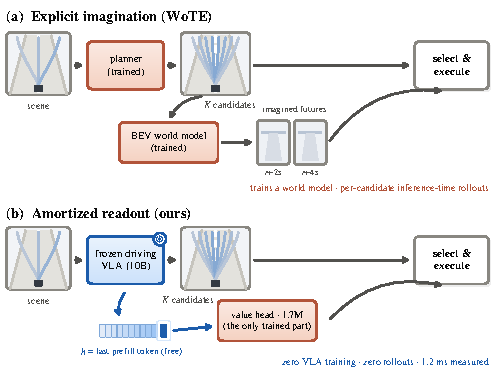
\includegraphics[width=\linewidth]{figs/fig1_teaser.pdf}
  \caption{\textbf{Two routes to online trajectory evaluation.}
  \emph{Top (explicit imagination, WoTE~\cite{li2025wote}):} a purpose-trained BEV world model autoregressively rolls out each candidate's future, then scores the imagined states.
  \emph{Bottom (ours, amortized):} the frozen driving VLA's own prompt prefill---computed anyway to generate the candidates---already summarizes the scene; its last hidden token feeds a \EffParams-parameter value head that scores all $K{=}8$ candidates in \EffLtMedianMs\,ms with zero inference-time rollouts and zero VLA training.}
  \label{fig:teaser}
\end{figure}

\section{Related Work}
\label{sec:related}

\paragraph{Online trajectory evaluation.}
WoTE~\cite{li2025wote} is the closest prior line: alongside an end-to-end planner emitting 256 K-Means anchor trajectories, it trains a BEV world model that imagines each candidate's future BEV state two steps ahead ($t{+}2$s, $t{+}4$s) and scores the imagined futures with imitation plus simulation-derived submetric rewards (collision, drivable area, time-to-collision, comfort, progress).
Rule-based scorers such as PDM~\cite{dauner2023pdm} evaluate candidates with hand-built kinematic forecasts, and Hydra-MDP-style distillation~\cite{li2024hydramdp} amortizes a rule-based scorer into the planner during training.
We occupy the far end of this spectrum: \emph{zero} inference-time rollout steps and \emph{zero} purpose-trained dynamics---the consequence knowledge is read from representations the frozen generator computes anyway, and consequence prediction appears only as an auxiliary training signal whose deletion provably does not change the deployed scores (\cref{sec:head}).
Positioning the two ends as \emph{explicit imagination} versus \emph{amortized consequence knowledge} makes the trade explicit; intermediate designs (scoring a predicted future) remain untested and we discuss them in \cref{sec:discussion}.

\paragraph{End-to-end planning and multi-modal output.}
UniAD~\cite{hu2023uniad}, VAD~\cite{jiang2023vad}, TransFuser~\cite{chitta2022transfuser}, and probabilistic-planning variants such as VADv2~\cite{chen2024vadv2} report minADE/minFDE-style metrics or best-of-$K$ closed-loop scores, inheriting the oracle-selector assumption from the trajectory-prediction literature~\cite{chai2019multipath}.
Closed-loop benchmarks~\cite{caesar2021nuplan,dauner2024navsim,jia2024bench2drive} score the executed trajectory, but public leaderboards rarely isolate how much of the headroom between executed and best-of-$K$ is recoverable by a better selector.
Our selected-regret endpoint measures exactly that recoverable gap under the deployed decision rule.

\paragraph{Frozen foundation-model representations.}
Linear probes~\cite{alain2016probes} and frozen-backbone transfer~\cite{lu2022fpt} established that pretrained representations support downstream readout without finetuning; driving VLAs~\cite{tian2024drivevlm,hwang2024emma,alpamayo2025} are typically consumed through their \emph{outputs} (trajectories, language) rather than their internal states.
To our knowledge this is the first work to (i) reuse a production driving VLA's internal prefill state for closed-loop trajectory selection, (ii) tie the reused representation bit-exactly to the candidate-generating forward pass, and (iii) support the reuse claim with causal ablations and prospective replication rather than correlational probing alone.

\paragraph{Evaluation rigor.}
Preregistration and adequately powered confirmatory designs are standard in clinical research and have been advocated for ML~\cite{vanmiltenburg2021preregistering,raff2019reproducibility}, but remain rare in autonomous-driving evaluation, where small effects on strong generators are easily manufactured---or missed---by analysis flexibility.
Every confirmatory claim in this paper is backed by a preregistered design with frozen gates, locked predictions, and paired scene bootstrap CIs~\cite{efron1994bootstrap}; \cref{sec:program} describes the program and \cref{tab:ladder} its cohort ladder.

\section{Method}
\label{sec:method}

\subsection{Setting}
\label{sec:setting}

We work in \simname, an internal high-fidelity closed-loop driving simulator whose \emph{official scene score} $y\in[0,1]$ aggregates safety, compliance, and progress into a single scalar per rollout.
The official score is the \emph{sole} selection supervision: submetric aggregates are deliberately barred from the selector's objective to prevent the selector from gaming individual submetrics---consequence submetrics enter only as auxiliary heads (\cref{sec:head}).
Each scene contributes three \emph{decision groups} at staggered decision times (timing tags A/B/C).
For each group, the frozen generator \vlaname{} (10B) samples $K{=}8$ candidate trajectories from one prompt prefill; every candidate is then executed in closed loop and receives its own official score, giving $3\times8=24$ scoring rollouts per scene and \nScoresTotal{} candidate-level scores on the \nScenes-scene primary cohort (\nGroups{} groups).

Given a group $g$ with candidates $c_1,\dots,c_K$ and scores $y(c_k)$, a selector $\pi$ picks $\hat c=\pi(g)$.
Our two co-primary endpoints are
\emph{selected regret}, $\regret(g) = \max_k y(c_k) - y(\hat c)$ (lower is better; the oracle-selector gap actually paid at deployment), and
\emph{tie-aware top-1 agreement}, $\mathbf{1}[\,y(\hat c) \ge \max_k y(c_k) - \epsilon\,]$ with $\epsilon=\TieEps$ (higher is better).
Both aggregate group $\rightarrow$ scene mean (3 groups) $\rightarrow$ seed mean $\rightarrow$ paired scene bootstrap (\cref{sec:protocol}).

\subsection{Same-prefill capture}
\label{sec:capture}

A representation-reuse claim is confounded if the representation could come from a \emph{different} forward pass than the candidates (different context window, different preprocessing, silently re-run prefill).
We eliminate this by construction: a capture hook inside the production \texttt{predict()} path records the final transformer layer's hidden states (post final normalization) of the prompt prefill, $H\in\mathbb{R}^{3086\times4096}$ (the prompt length is invariant across groups), \emph{during the same call} that samples the $K$ candidates, with an exactly-one-prefill assertion so a second prefill in the call would fail the capture rather than silently substitute context.
The pooled scene vector used at deployment is the last row, $h = H_{3086}\in\mathbb{R}^{4096}$; capture-time SHA-256 hashes of both tensors establish bit-exact provenance ($h \equiv H[-1]$ verified for \nGroups/\nGroups{} groups), and every downstream artifact (training tables, locked predictions, analysis JSONs) carries these hashes forward.
\Cref{fig:capture} summarizes the chain.
Candidates, representation, and scores are therefore certifiably co-produced---the ablations in \cref{sec:res-signal} then test whether the representation's \emph{content} matters.

\begin{figure}[t]
  \centering
  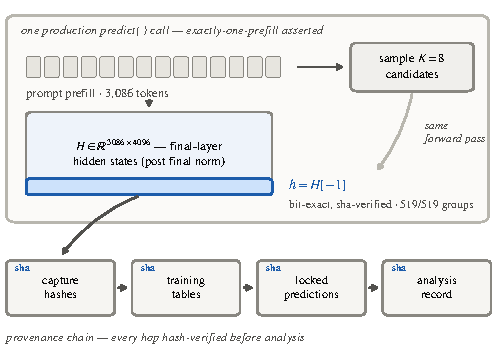
\includegraphics[width=\linewidth]{figs/fig_capture.pdf}
  \caption{\textbf{Same-prefill capture and provenance.} One production \texttt{predict()} call per decision group: the 3{,}086-token prompt prefill produces both the $K{=}8$ sampled candidates and the captured final-layer hidden states $H$; the deployed scene vector is bit-exactly $h=H[-1]$ (SHA-256 verified at capture, \nGroups/\nGroups{} groups). Every downstream artifact---training tables, locked predictions, the analysis record---carries the hashes forward.}
  \label{fig:capture}
\end{figure}

\subsection{Selector head}
\label{sec:head}

\begin{figure*}[t]
  \centering
  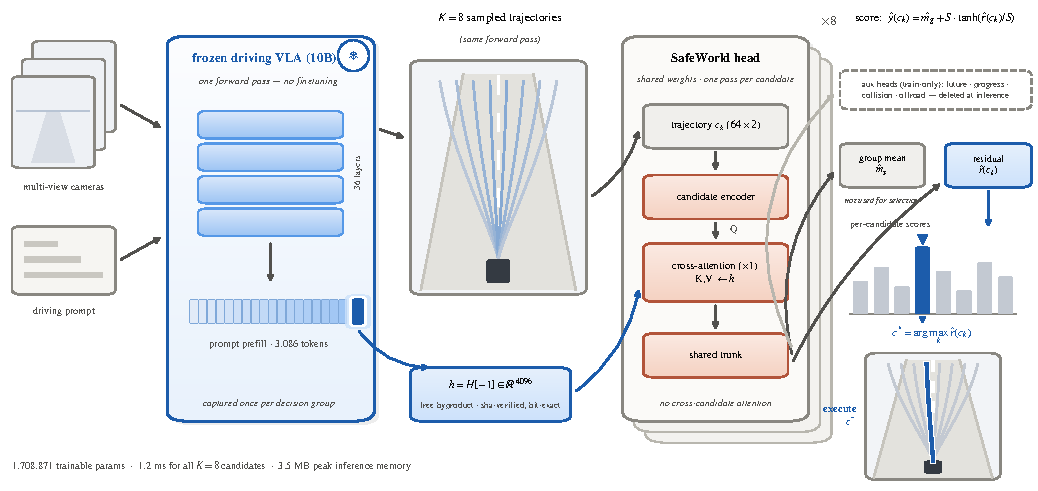
\includegraphics[width=\textwidth]{figs/fig_arch.pdf}
  \caption{\textbf{Architecture.} One frozen forward pass of \vlaname{} yields both the $K{=}8$ candidate trajectories and the prefill hidden states $H$; the only representation consumed downstream is the last row $h=H[-1]$, a free byproduct of generation. The \headname{} head (\EffParams{} parameters---the only trained component) runs once per candidate with shared weights: a candidate encoder queries $h$ through a single cross-attention block into a shared trunk. The score decomposes into a group mean $\hat m_g$ (excluded from selection) and a bounded residual $\hat r$ that alone drives the selector (\cref{eq:decomp}); the selected trajectory is executed. Auxiliary consequence heads are training-only---deleted at inference, the deployed score is bit-identical. Per-candidate scores and trajectories in the panel are illustrative.}
  \label{fig:arch}
\end{figure*}

The \headname{} head (\cref{fig:arch}; \EffParams{} trainable parameters; the frozen VLA receives no gradients) scores each candidate independently---no cross-candidate attention, so scores are $K$-invariant and permutation-equivariant by construction (verified: off-diagonal cross-candidate gradients are exactly zero; scores are bit-identical alone or batched).
A candidate encoder embeds the trajectory; a single cross-attention block queries the scene representation (the last token $h$, or in ablation arms the full sequence $H$); shared trunk features feed the output heads.

\paragraph{Decomposed score.}
Naively regressing $y$ conflates two signals of very different scale: the group's overall difficulty and the candidate's \emph{relative} quality within the group---and only the latter matters for selection.
Earlier design-phase studies in this program showed the conflation concretely: an unconstrained residual develops gradient conflict between ranking and centered-regression losses, and group-level offsets dominate the representation.
We therefore decompose
\begin{equation}
  \hat y(c) \;=\; \hat m_g \;+\; S\,\tanh\!\big(\hat r(c)/S\big),
  \qquad S=0.67,
  \label{eq:decomp}
\end{equation}
where $\hat m_g$ is a group-mean head, $\hat r(c)$ is a per-candidate residual (zero-initialized), and the bound $S$ (frozen from development-cohort residual statistics) keeps the residual inside the empirically observed spread.
The deployed selector is $\hat c=\arg\max_c \hat r(c)$: the group-mean head is excluded from selection by construction, so scene difficulty cannot leak into the choice.

\paragraph{Amortized consequence knowledge.}
Auxiliary heads predict per-candidate consequences: future ego trajectory ($64\times2$), progress, collision, and offroad.
They are \emph{training-only}: at inference the deployed score is bit-identical with the auxiliary heads deleted (a deletion test in the conformance suite).
This is the operational sense in which the selector holds \emph{amortized} world knowledge---consequences shape the representation during training but are never simulated, predicted, or consumed at decision time, in contrast to explicit-imagination designs~\cite{li2025wote}.

\subsection{Objectives}
\label{sec:objectives}

All representation arms share one architecture and parameter count (state dicts are interchangeable); arms differ only in scene-input visibility and objective.
The \emph{checkpoint objective} (used by all arms for model selection during training) is
$L = 1.0\,L_{\text{rank}} + 0.5\,L_{\text{centered}} + 0.1\,L_{\text{group-mean}} + 0.25\,L_{\text{future}} + 0.1\,L_{\text{progress}} + 0.1\,L_{\text{collision}} + 0.1\,L_{\text{offroad}}$,
with a weighted pairwise softplus ranking loss and scale-matched SmoothL1 regressions.

\paragraph{Selector loss.}
Ranking all $K$ candidates well is not the deployed task; putting the \emph{best} candidate on top is.
The selector objective replaces $L_{\text{rank}}$ (coefficient moved to 0) with a regret-weighted best-vs-rest logistic loss.
With tied-best set $B_g=\{i: y_{\max}-y_i\le\epsilon\}$ and per-candidate selector scores $s$,
\begin{equation}
  L_{\text{sel}} \;=\; \frac{\sum_{g}\sum_{i\in B_g}\sum_{j\notin B_g} \frac{w_j}{|B_g|}\,
  \mathrm{softplus}\!\big({-}(s_i-s_j)/\tau\big)}{\sum_g \sum_{j\notin B_g} w_j},
  \qquad w_j = y_{\max}-y_j,
  \label{eq:selloss}
\end{equation}
so each mistake is weighted by exactly the regret it would cost.
Both scalars are resolved \emph{mechanically} from frozen target metadata, not tuned: $\tau=\SelTau$ is the (0.001-ceiled) median positive oracle-best-to-candidate score gap, and the coefficient $\SelCoef$ equalizes the RMS per-candidate gradient $\partial L/\partial s$ against the replaced ranking term at equal scores.

\paragraph{Why not expected regret?}
The natural alternative---minimizing the expected regret of a softmax policy, $L_A=\mathbb{E}_{q}[r]$ with $q=\mathrm{softmax}(s/\tau)$---was rejected on a closed, preregistered criterion: its gradient $\partial L_A/\partial s_j = \tfrac{1}{\tau}q_j(r_j-\mathbb{E}_q[r])$ \emph{vanishes} as $q$ collapses onto a single candidate, i.e.\ exactly when the selector is \emph{confidently wrong}---the one failure mode the objective exists to repair.
The best-vs-rest logistic instead \emph{saturates at its maximum} there.
In the operating regime our development runs actually produce (within-group score spreads routinely $2.6$--$10\times$ $\tau$), the softmax gradient retains as little as $3.9\%$ of its small-spread magnitude; reproduced synthetically in the preregistration conformance suite, the softmax gradient norm collapses to \SelGradVanish{} while the frozen selector loss holds \SelGradSat.
This geometry, not any real-model outcome comparison, fixed the objective before the confirmatory studies ran (derivation and the full 12-criterion resolution in the supplement).

\subsection{Protocol}
\label{sec:protocol}

Every confirmatory study follows one frozen protocol.
\textbf{Training/evaluation:} 5-fold cross-validation split by scene $\times$ 3 seeds; checkpoint selection uses \emph{inner-validation only} (\textsc{constrained-selector-first} rule; the test fold is never consulted).
\textbf{Locking:} all per-candidate predictions for every arm and every ablation condition are hash-locked \emph{before} any endpoint is computed; the analyzer verifies every hash (and its own code hash against the registered one) and runs exactly once.
\textbf{Statistics:} paired scene percentile bootstrap, $10{,}000$ resamples, frozen seed; undefined scenes are dropped and counted, never zero-filled; we report 95\% CIs throughout and treat an effect as supported only when its CI excludes zero.
\textbf{Preregistration:} arms, endpoints, gates, margins, ablation mappings, and analysis code are frozen and hash-registered before outcomes exist; deviations would be visible as hash breaks.

\section{Experimental Program}
\label{sec:program}

We treat the evaluation design itself as a contribution: selector effects on strong generators are small, and without preregistration and cohort discipline they are easy to manufacture.
This section fixes the vocabulary used in \cref{sec:results}.

\paragraph{Cohort ladder.}
Scenes advance through four rungs (\cref{tab:ladder}).
Development scenes absorbed all architecture and objective design, including every repair and failed branch.
The \emph{prospective untouched} cohort (\nScenes{} scenes, \nGroups{} groups, \nScoresTotal{} candidate scores) was frozen outcome-blind---captured, hashed, and quarantined before any model consumed it---and first opened by the confirmatory matched-visibility study of \cref{sec:res-signal,sec:res-onetoken}.
The \emph{extension} cohort (+\FnNNew{} scenes target) exists solely to power the incumbent study of \cref{sec:res-incumbent}.
A \emph{sealed} 35-scene cohort is never opened until a winner is frozen; it exists to confirm a promoted selector once, or to stay sealed.

\begin{table}[t]
  \centering
  \small
  \begin{tabular}{@{}llll@{}}
    \toprule
    Rung & Scenes & Role & Status \\
    \midrule
    Development & 122 & design, repairs & opened freely \\
    Prospective & \nScenes{} & confirmatory M-study & frozen, used once \\
    Extension & +\FnNNew{} & powered N-study & \iffnonedone consumed \else in acquisition \fi \\
    Sealed & 35 & one-shot confirmation & never opened \\
    \bottomrule
  \end{tabular}
  \caption{\textbf{Cohort ladder.} Each rung is hash-frozen before use; registered preregistration digests for each stage are listed in the supplement.}
  \label{tab:ladder}
\end{table}

\paragraph{Endpoints.}
Selected regret and tie-aware top-1 agreement at $K{=}8$ (co-primary; $K{=}2/5$ secondary, first-$k$ subsets in the frozen candidate order) as defined in \cref{sec:setting}.
Selected regret is exactly the slack that minADE@$K$-style reporting hides: the gap between the best available candidate's outcome and the outcome of the candidate the deployed rule picks.
Reporting both endpoints matters because they can disagree---a selector can pick near-best candidates reliably (low regret) while losing exact-best agreement, and vice versa; we will see precisely this tension in \cref{sec:res-incumbent}.

\paragraph{Arms.}
Four selectors, identical labels and folds:
\Ltok{} reads the last prefill token $h$;
\Lfull{} reads the full sequence $H$ (parameter-matched to \Ltok, interchangeable state dicts);
\Lnull{} is the matched scene-blind control---the scene input is a single zero token (no learned null embedding), so the arm retains the identical graph and capacity but no scene information;
\Lgeo{} is the trained incumbent: a trajectory-geometry-only MLP ($\sim$202k parameters, its own frozen historical objective) that sees no VLA representation at all.
The confirmatory matched-visibility study compares
M1 $=$ \Lfull$-$\Ltok,
M2 $=$ \Lfull$-$\Lnull,
M3 $=$ \Ltok$-$\Lnull,
M4 $=$ \Lfull$-$\Lgeo,
M5 $=$ \Ltok$-$\Lgeo{}
(paired per scene, 3 seeds each).

\paragraph{Causal ablations.}
On the representation-reading arm, at inference time and with the training entirely untouched:
\textsc{wrong-scene} substitutes the representation of a different scene under a preregistered donor mapping;
\textsc{zero} zeroes the representation;
a \textsc{last-token-only} diagnostic feeds the \Lfull{} reader just the final row.
If the selection signal genuinely lives in the scene representation's \emph{content}, the first two must degrade selection; if the \Lfull{} reader actually consumes the sequence, the third must degrade \emph{it}.

\paragraph{The powered incumbent study.}
The matched-visibility study leaves \Ltok{} vs.\ \Lgeo{} unresolved at $N{=}\nScenes$ (\cref{sec:res-incumbent}); its point effect defines the minimum detectable effect for a follow-up sized \emph{before} outcomes: MDE $=\FnMde$ regret (the locked M5 point estimate, recomputed bit-exactly from locked predictions), paired scene SD $\FnSdPaired$, two-sided $\alpha=0.05$, $1-\beta=0.80$ $\Rightarrow$ $N=\FnNTotal$ analysis scenes ($\FnNExisting$ existing $+$ \FnNNewPreAttrition{} new, acquired as \FnNNew{} with a 20\% attrition allowance; achieved power \FnPowerAchieved; top-1 MDE \FnTopOneMde).
Four arms are preregistered---\Ltok{} under the checkpoint objective and under the selector objective (\cref{sec:objectives}), \Lnull, and \Lgeo---with a frozen selector-first nomination rule and comparison graph
N1 $=$ nominated$-$\Lgeo{} (promotion),
N2 $=$ nominated$-$\Lnull{} (M3 replication at scale),
N3 $=$ selector$-$checkpoint objective (the controlled selector-loss contrast),
N4 $=$ checkpoint$-$\Lgeo{} (always reported).
Promotion requires ten frozen gates (regret superiority with CI support, top-1 and pairwise non-inferiority at frozen margins, causal-ablation behavior, $K$-consistency, seed/fold/leave-one-scene-out robustness including consistency on the untouched extension subset alone, deployment budget, and integrity checks); the full gate table with margins is in the supplement.

\section{Results}
\label{sec:results}

All confirmatory numbers in this section are computed once from hash-locked predictions on the prospective untouched cohort (\nScenes{} scenes; paired scene bootstrap, 95\% CIs) and are machine-read from the locked analysis records into this manuscript.
\Cref{tab:main} reports absolute levels and paired contrasts; \cref{fig:results} plots every primary contrast.

\begin{table*}[t]
  \centering
  \small
  \begin{subtable}{0.44\textwidth}
    \centering
    \begin{tabular}{@{}lccc@{}}
      \toprule
      Arm & Regret $\downarrow$ & Top-1 $\uparrow$ & Pairwise $\uparrow$ \\
      \midrule
      \Lnull{} (scene-blind) & \AbsNullKEightRegret & \AbsNullKEightTopOne & \AbsNullKEightPairwise \\
      \Lgeo{} (incumbent) & \AbsLegacyKEightRegret & \AbsLegacyKEightTopOne & \AbsLegacyKEightPairwise \\
      \Lfull{} (sequence) & \AbsFullKEightRegret & \AbsFullKEightTopOne & \AbsFullKEightPairwise \\
      \Ltok{} (ours) & \textbf{\AbsLasttokenKEightRegret} & \AbsLasttokenKEightTopOne & \AbsLasttokenKEightPairwise \\
      \bottomrule
    \end{tabular}
    \caption{Absolute levels @$K{=}8$ (scene-macro means).}
    \label{tab:main-abs}
  \end{subtable}
  \hfill
  \begin{subtable}{0.53\textwidth}
    \centering
    \begin{tabular}{@{}llll@{}}
      \toprule
      Contrast & $\Delta$Regret $\downarrow$ [95\% CI] & $\Delta$Top-1 $\uparrow$ [95\% CI] \\
      \midrule
      M3: \Ltok$-$\Lnull & \MThreeKEightRegretCI & \MThreeKEightTopOneCI \\
      M2: \Lfull$-$\Lnull & \MTwoKEightRegretCI & \MTwoKEightTopOneCI \\
      M1: \Lfull$-$\Ltok & \MOneKEightRegretCI & \MOneKEightTopOneCI \\
      M5: \Ltok$-$\Lgeo & \MFiveKEightRegretCI & \MFiveKEightTopOneCI \\
      M4: \Lfull$-$\Lgeo & \MFourKEightRegretCI & \MFourKEightTopOneCI \\
      \bottomrule
    \end{tabular}
    \caption{Paired scene contrasts @$K{=}8$ (negative regret / positive top-1 favor the first-named arm).}
    \label{tab:main-delta}
  \end{subtable}
  \caption{\textbf{Main endpoints on the prospective untouched cohort} (\nScenes{} scenes, \nGroups{} groups, 3 seeds). Bold marks the best regret. CIs from paired scene bootstrap ($10{,}000$ resamples). M3 establishes the scene signal (both CIs exclude zero); M1 establishes that the full sequence is \emph{worse} than its last token (both CIs exclude zero); M5 motivates the powered study of \cref{sec:res-incumbent} (both CIs cross zero).}
  \label{tab:main}
\end{table*}

\begin{figure}[t]
  \centering
  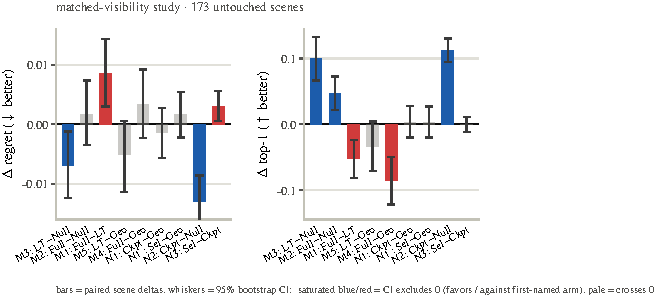
\includegraphics[width=\linewidth]{figs/fig_results.pdf}
  \caption{\textbf{All primary contrasts} ($K{=}8$ selected regret left, tie-aware top-1 right; bars are paired scene deltas, whiskers 95\% bootstrap CIs, drawn directly from the locked analysis records). Saturated blue/red: CI excludes zero, favoring / opposing the first-named arm; pale gray: CI crosses zero. M1--M5: matched-visibility study\iffnonedone; N1--N4: powered incumbent study\else{} (N1--N4 of the powered incumbent study are in flight)\fi.}
  \label{fig:results}
\end{figure}

\subsection{The scene signal is real, and causal}
\label{sec:res-signal}

The paired contrast that isolates scene information---\Ltok{} versus the graph- and parameter-identical scene-blind \Lnull---is CI-supported on \emph{both} co-primary endpoints: selected regret \MThreeKEightRegretCI{} and top-1 agreement \MThreeKEightTopOneCI{} (\cref{tab:main}, M3), on scenes no model in the program had ever consumed.
In absolute terms the last-token selector recovers regret from \AbsNullKEightRegret{} to \AbsLasttokenKEightRegret{} and lifts exact-best agreement from \AbsNullKEightTopOne{} to \AbsLasttokenKEightTopOne; secondary endpoints agree (pairwise ranking accuracy \MThreeKEightPairwiseCI; top-1 at $K{=}5$: \MThreeKFiveTopOneCI, $K{=}2$: \MThreeKTwoTopOneCI).
The effect replicates the direction and magnitude first observed on development scenes during the design phase, making this its first \emph{prospective} confirmation on an untouched cohort.\todo{supp: add the development-phase (E1) record values as the internal-replication table}

Correlation with scene content, not just presence of \emph{some} input, is established by inference-time ablations on the sequence-reading arm (\cref{fig:ablations}): substituting a \emph{different} scene's representation degrades top-1 by \AblWrongSceneTopOneCI, and zeroing it degrades top-1 by \AblZeroSceneTopOneCI---both CIs excluding zero---while regret shifts stay small (\AblWrongSceneRegretCI{} and \AblZeroSceneRegretCI, CIs crossing zero) with no contradictory material improvement on either endpoint.
The degradation concentrating on top-1 is the expected signature: scene content is what disambiguates near-tied candidates at the top of the list.

The full-sequence arm corroborates the signal's existence from a second angle: \Lfull{} also beats \Lnull{} on top-1 (\MTwoKEightTopOneCI, M2)---the sequence \emph{contains} the information---which sharpens the next finding: the failure of \Lfull{} is about \emph{form}, not existence.

\begin{figure}[t]
  \centering
  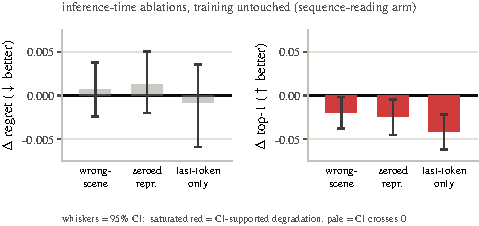
\includegraphics[width=\linewidth]{figs/fig4_ablations.pdf}
  \caption{\textbf{Causal ablations} (inference-time, training untouched; deltas vs.\ the arm's NORMAL condition @$K{=}8$, 95\% CIs). Wrong-scene substitution and zeroing degrade top-1 (CIs exclude zero); the last-token-only diagnostic degrades the \Lfull{} reader (top-1 \AblLastTokenDiagTopOneCI), showing it genuinely consumes sequence positions---yet it still loses to the last-token-trained arm end-to-end (\cref{sec:res-onetoken}).}
  \label{fig:ablations}
\end{figure}

\subsection{One token beats the sequence}
\label{sec:res-onetoken}

Giving the reader the entire $3{,}086\times4{,}096$ prefill---strictly more information than its last row, under an identical parameter budget (\EffParams{} parameters, interchangeable state dicts)---makes selection \emph{worse}, with CI support on both primaries: regret \MOneKEightRegretCI{} and top-1 \MOneKEightTopOneCI{} (\cref{tab:main}, M1).
The deficit is consistent, not a $K{=}8$ artifact: top-1 at $K{=}5$ \MOneKFiveTopOneCI{} and $K{=}2$ \MOneKTwoTopOneCI, pairwise accuracy \MOneKEightPairwiseCI.

Two probes localize the mechanism.
First, the \Lfull{} reader did \emph{not} degenerate into a last-token reader: feeding it only the final row at inference costs it a further \AblLastTokenDiagTopOneCI{} top-1---it genuinely attends across the sequence.
The cost is therefore paid at \emph{training} time: spreading a fixed-capacity reader's cross-attention over 3{,}086 tokens yields a worse selection function than concentrating it on the one token where the generator has already aggregated the scene---the state from which it began emitting candidates.
Second, the auxiliary consequence heads split: \Lfull{} is CI-supported \emph{worse} on future-trajectory ADE (\AuxAdeCI) and collision AUROC (\AuxCollisionCI; $n{=}\AuxCollisionNScenes$ scenes with defined labels) but CI-supported \emph{better} on FDE (\AuxFdeCI).
Sequence access is not uniformly useless---it helps some long-horizon geometry---but the \emph{selection-relevant} summary is best read where the generator itself deposited it.
Under matched parameters, explanations based on reader capacity are excluded by design; what remains is information accessibility.
For practitioners the implication is blunt: the cheapest representation (one token, \EffMemRatio$\times$ less memory than the sequence; \cref{sec:res-eff}) is also the right one.

\subsection{The incumbent test at adequate power}
\label{sec:res-incumbent}

Against the trained geometry incumbent, the matched-visibility study ends in tension (\cref{tab:main}, M5): the representation arm leads on regret (\MFiveKEightRegretCI) while the incumbent leads on exact-best agreement (\MFiveKEightTopOneCI)---absolute top-1 \AbsLegacyKEightTopOne{} vs.\ \AbsLasttokenKEightTopOne---and \emph{both} CIs cross zero.
At $N{=}\nScenes$ this comparison is simply underpowered for the observed effect; concluding either way would be exactly the practice \cref{sec:program} is designed to prevent.
We therefore preregistered a consolidation study sized for it: $N=\FnNTotal$ scenes gives $1-\beta=\FnPowerAchieved$ at two-sided $\alpha=0.05$ for the locked MDE (\FnMde{} regret), with all arms, gates, margins, nomination order, and analysis code frozen before any new scene was scored.

\iffnonedone
\iffnonepass
The nominated representation selector \textbf{passes}: N1 regret \NOneKEightRegretCI{} (CI-supported superiority over \Lgeo) with top-1 non-inferiority satisfied (\NOneKEightTopOneCI{} against frozen margins), and the scene-value contrast replicates at scale (N2 regret \NTwoKEightRegretCI, top-1 \NTwoKEightTopOneCI) on \FnOneNScenes{} scenes.
The checkpoint-objective candidate is reported alongside (N4 regret \NFourKEightRegretCI, top-1 \NFourKEightTopOneCI).
\todo{fill gate-by-gate outcomes + per-cohort consistency clause from the FN1 record; update \cref{fig:results}}
\else
The nominated representation selector \textbf{does not displace the incumbent}: N1 regret \NOneKEightRegretCI{} on \FnOneNScenes{} scenes fails the preregistered superiority gate\todo{state which gate(s) failed, from the FN1 record}, while the scene-value contrast N2 (regret \NTwoKEightRegretCI, top-1 \NTwoKEightTopOneCI) \todo{state whether M3 replicated at scale}.
We report this as a \emph{boundary result} with unusual evidential value: at $0.80$ power, the frozen representation demonstrably adds scene information a geometry selector lacks (\cref{sec:res-signal}, and N2 at scale), yet that information is not sufficient to beat a well-tuned geometry baseline on the promoting endpoint at the effect size that motivated the study.
Representation reuse pays when no tuned incumbent exists or when top-of-list disambiguation (where the scene signal concentrates) is the binding constraint; it does not automatically retire strong geometric priors.
The checkpoint-objective candidate behaves consistently (N4 regret \NFourKEightRegretCI, top-1 \NFourKEightTopOneCI).
\fi
\else
The study is in flight at submission-preparation time: the extension cohort is in acquisition under the frozen protocol, and both outcome branches of this subsection are pre-written against the registered gates. \todo{FN1 finalizes $\sim$Aug 10--11: flip \texttt{\textbackslash fnonedone}/\texttt{\textbackslash fnonepass} in main.tex, run \texttt{make\_numbers.py --fn1}, delete this placeholder paragraph.}
\fi

\subsection{Does the selector loss buy the top of the list?}
\label{sec:res-selloss}

The controlled contrast N3 isolates the objective of \cref{eq:selloss}: same architecture, same data, rank term replaced by the regret-weighted best-vs-rest logistic.
The preregistered success criterion is asymmetric by design---the selector loss must \emph{buy} top-1 (CI above zero) without \emph{selling} regret (CI upper bound below $+0.005$)---because the design-phase precedent showed a large top-1 gain (${\sim}{+}0.08$) at a small regret concession.\todo{supp: cite exact E1 record values}
\iffnonedone
N3 lands at top-1 \NThreeKEightTopOneCI{} and regret \NThreeKEightRegretCI: \iffnonepass the trade clears the gate, and the selector-objective candidate is the nominated arm reported above.\else\ \todo{write the observed verdict: gate cleared / not cleared, and which candidate was nominated}\fi
\else
\fnpending
\fi

\subsection{Efficiency}
\label{sec:res-eff}

\Cref{tab:eff} summarizes deployment cost on a single workstation GPU.
The deployed configuration---last token in, all $K{=}8$ candidates scored---runs in \EffLtMedianMs{}\,ms median (\EffLtTailMs{}\,ms p95) with \EffLtMemMb{}\,MB peak incremental memory and \EffParams{} trainable parameters, orders of magnitude under the preregistered ceilings (\EffCeilMedianMs/\EffCeilTailMs\,ms, \EffCeilMemGb\,GiB, \EffCeilParams{} params).
The representation itself is free: it is a byproduct of the prefill that generates the candidates.
No VLA finetuning, no world model, no inference-time rollouts; the entire selector trains in minutes (peak \EffTrainPeakMb\,MB per worker).
For contrast, the full-sequence reader needs \EffFullMemMb{}\,MB at inference (\EffMemRatio$\times$ more) and is \emph{worse} (\cref{sec:res-onetoken}); explicit-imagination designs additionally pay for a purpose-trained world model and its inference-time rollouts, a cost class our amortized route avoids entirely.

\begin{table}[t]
  \centering
  \small
  \begin{tabular}{@{}lrrr@{}}
    \toprule
    & Params & Latency (med/p95) & Peak mem \\
    \midrule
    \Ltok{} head (deployed) & \EffParams & \EffLtMedianMs{}/\EffLtTailMs{}\,ms & \EffLtMemMb{}\,MB \\
    \Lfull{} reader & \EffParams & \EffFullMedianMs{}/\EffFullTailMs{}\,ms & \EffFullMemMb{}\,MB \\
    \midrule
    Preregistered ceiling & \EffCeilParams & \EffCeilMedianMs{}/\EffCeilTailMs{}\,ms & \EffCeilMemGb{}\,GiB \\
    \bottomrule
  \end{tabular}
  \caption{\textbf{Deployment cost} (incremental over the generator, all $K{=}8$ candidates, bf16, single workstation GPU; 200 timed iterations).}
  \label{tab:eff}
\end{table}

\iffnonepass
\subsection{Sealed-cohort confirmation}
\label{sec:res-sealed}
Following promotion, the 35-scene sealed cohort---never opened by any stage of the program---was unsealed exactly once. \todo{FN2: fill when/if it exists.}
\fi

\section{Discussion and Limitations}
\label{sec:discussion}

\paragraph{Internal benchmark, by choice.}
All results are measured in \simname{} against its official closed-loop score; they are not comparable to NavSim, nuPlan, or Bench2Drive leaderboards~\cite{dauner2024navsim,caesar2021nuplan,jia2024bench2drive}, and we claim no state of the art.
The trade was deliberate: closed-loop official scoring of \emph{every} candidate (not just the executed one) is what makes selected regret directly measurable, and a controlled internal environment is what makes prospective freezing, sealed cohorts, and bit-exact provenance enforceable.
We give up leaderboard placement and buy inferential validity; porting the protocol to a public closed-loop benchmark is the obvious next step and the capture contract (\cref{sec:capture}) is simulator-agnostic.

\paragraph{Small absolute effects are the honest scale.}
A regret delta of \MThreeKEightRegretMean{} on a $[0,1]$ score is small.
That is what selection headroom under a strong generator at $K{=}8$ \emph{is}: the incumbent already operates near the oracle on most groups, and the remaining slack concentrates in a minority of scenes.
This is precisely why the paper leans on CIs, preregistration, and a powered design rather than point estimates---at this effect scale, standard practice (single split, no CIs, post-hoc metric choice) can produce any conclusion one likes.
We regard the evidence standard as load-bearing for the claims, not as ornamentation.

\paragraph{Scope.}
One generator (\vlaname, 10B), one simulator, one candidate regime ($K{=}8$ sampled; WoTE-style designs use up to 256 anchors), one representation site (final-layer prefill).
The last-token result is a statement about \emph{this} class of autoregressive driving VLAs---where the prefill terminus is the state from which generation begins---and its transfer to other architectures (e.g., diffusion planners with no comparable terminus) is untested.
Scenes are simulator-native; no real-world driving data is touched.

\paragraph{The amortized--explicit spectrum.}
Our zero-rollout endpoint and WoTE's online imagination bracket a spectrum whose middle is unexplored: scoring a \emph{predicted} future (one amortized rollout step), consuming the auxiliary heads at inference, or distilling an explicit evaluator into a prefill reader.
The deletion test (\cref{sec:head}) gives the spectrum a crisp operational coordinate: how much of the evaluator's decision changes when its forward-looking components are removed at inference.
Mapping selection quality along that coordinate---and testing whether the last-token summary remains sufficient as $K$ grows toward anchor-set scale---is where we would go next.

{
    \small
    \bibliographystyle{ieeenat_fullname}
    \bibliography{main}
}

\end{document}
